\documentclass[aps,prb,twocolumn,superscriptaddress,footinbib,amsmath,amssymb,floatfix]{revtex4}
%\documentclass[aps,prb,onecolumn,preprint,superscriptaddress,footinbib,amsmath,amssymb,floatfix]{revtex4}
\usepackage[dvips]{epsfig}
\usepackage{graphicx}
\usepackage{ifthen}
\usepackage{dcolumn}% Align table columns on decimal point
\usepackage{bm}% bold math
\usepackage{multirow}
\usepackage{booktabs}
\usepackage{bm}% bold math
\usepackage{amsbsy}
\usepackage{amsmath}
\usepackage{amssymb}
\usepackage{subfigure}
\usepackage{xcolor}
%\usepackage{wrapfig}

%Definition of new commands
\newcommand{\f}[2]{\ensuremath{\frac{\displaystyle{#1}}{\displaystyle{#2}}}}
\newcommand{\lr}[1]{\langle{#1}\rangle}
\newcommand{\colv}[2] {\left(\begin{array}{c} #1 \\ #2 \end{array}\right)}
\renewcommand{\thefootnote}{\fnsymbol{footnote}}
\newcommand{\be} {\begin{eqnarray}}
\newcommand{\ee} {\end{eqnarray}}
%--------------------------------------------------------------------------
%EQ COMMANDS
%--------------------------------------------------------------------------
\newcommand{\two}{\mspace{-2.0mu}}
\newcommand{\four}{\mspace{-4.0mu}}
\newcommand{\plus}{\mspace{-4.5mu}+\mspace{-3.5mu}}
\newcommand{\minus}{\mspace{-4.5mu}-\mspace{-3.5mu}}
\newcommand{\pp}{'\mspace{-2.0mu}'}
\newcommand{\xlb}[4]{#1\ifthenelse{\equal{#2}{0}}{}{_{\alpha #2}}
\mspace{-2.0mu}\genfrac{(}{)}{0pt}{1}{\ifthenelse{\equal{#3}{0}}{0}{l #3}} 
{\ifthenelse{\equal{#4}{0}}{0}{b #4}}}

\newcommand{\xkv}[4]{#1\mspace{-5.0mu}\left(\mspace{-8.0mu}
\begin{smallmatrix}#2\four{}\four{}\mspace{-8.0mu}&\pmb{\kappa}#3\\&\nu 
#4\end{smallmatrix}\mspace{-5.0mu}\right)}

\newcommand{\evect}[6]{#1\mspace{-4.0mu}\left(\mspace{-8.0mu}
\begin{smallmatrix}#2\mspace{-8.0mu}&\pmb{\kappa} #3 &b #5\\&\nu #4 &
\alpha #6\end{smallmatrix}\mspace{-5.0mu}\right)}

\newcommand{\varmat}[8]{\mspace{-5.0mu}\left(\mspace{-8.0mu}
\begin{smallmatrix}\ifthenelse{\equal{#3}{0}}{\mspace{-8.0mu}&b_{#1}&b_{#2}
\\&\alpha_{#1}&\alpha_{#2}} {\ifthenelse{\equal{#7}{0}}{#1\mspace{-8.0mu}&
\pmb{\kappa}#2#3\mspace{-8.0mu}&\pmb{\kappa}#4#5\mspace{-8.0mu}&\pmb{\kappa}
#6\\&\nu#2&\nu#4&\nu#6} {#1\mspace{-8.0mu}&\pmb{\kappa}#2#3\mspace{-8.0mu}&
\pmb{\kappa}#4#5\mspace{-8.0mu}&\pmb{\kappa}#6#7\mspace{-8.0mu}&\pmb{\kappa}
#8\\&\nu#2&\nu#4&\nu#6&\nu#8}}\end{smallmatrix}\mspace{-5.0mu}\right)}

\newcommand{\EXP}[1]{\exp\mspace{-5.0mu}\left[#1\right]\mspace{-3.0mu}}

\newcommand{\tpp}[2]{\left(\mspace{-2.0mu}\xkv{\omega}{}{}{}#1\xkv{\omega}
{}{'}{'}#2\xkv{\omega}{}{\pp}{\pp}\mspace{-2.0mu}\right)}



%--------------------------------------------------------------------------
\newcommand{\SUM}[2]{\ifthenelse{\equal{#1}{0}}{\sum_{
\alpha_{#2},b_{#2},l_{#2}}^{3,n,N}} {\ifthenelse{\equal{#1}{1}}{\sum_{
\alpha_{#2},b_{#2}}^{3,n}}{\sum_{\pmb{\kappa}#2,\nu#2}^{N,3n}}}}

\newcommand{\SUMprime}[2]{\ifthenelse{\equal{#1}{0}}
{\sum_{\alpha_{#2},b_{#2},l_{#2}}^{3,n,N}} 
{\ifthenelse{\equal{#1}{1}}{\sum_{\alpha_{#2},b_{#2}}^{3,n}}
{\sum_{\pmb{\kappa}^{'}#2,\nu#2}^{N,3n}}}}

\newcommand{\SUMalpha}[2]{\ifthenelse{\equal{#1}{0}}
{\sum_{\alpha_{#2}}^{3}} {\ifthenelse{\equal{#1}{1}}
{\sum_{\alpha_{#2},b_{#2}}^{3,n}}{\sum_{\pmb{\kappa}#2,\nu#2}^{N,3n}}}}
%--------------------------------------------------------------------------
\newcommand{\SUMalphap}[2]{\ifthenelse{\equal{#1}{0}}
{\sum_{\alpha'_{#2}}^{3}} {\ifthenelse{\equal{#1}{1}}
{\sum_{\alpha'_{#2},b'_{#2}}^{3,n}}{\sum_{\pmb{\kappa}#2,\nu#2}^{N,3n}}}}

\newcommand{\SUMb}[2]{\ifthenelse{\equal{#1}{0}}{\sum_{b_{#2}}^{n}}
 {\ifthenelse{\equal{#1}{1}}{\sum_{\alpha_{#2},b_{#2}}^{3,n}}
{\sum_{\pmb{\kappa}#2,\nu#2}^{N,3n}}}}

\newcommand{\SUMbp}[2]{\ifthenelse{\equal{#1}{0}}{\sum_{b'_{#2}}^{n}}
 {\ifthenelse{\equal{#1}{1}}{\sum_{\alpha'_{#2},b'_{#2}}^{3,n}}
{\sum_{\pmb{\kappa}#2,\nu#2}^{N,3n}}}}

\newcommand{\SUMl}[2]{\ifthenelse{\equal{#1}{0}}{\sum_{l_{#2}}^{N}}
 {\ifthenelse{\equal{#1}{1}}{\sum_{\alpha_{#2},b_{#2}}^{3,n}}
{\sum_{\pmb{\kappa}#2,\nu#2}^{N,3n}}}}

\newcommand{\SUMlp}[2]{\ifthenelse{\equal{#1}{0}}{\sum_{l'_{#2}}^{N}}
 {\ifthenelse{\equal{#1}{1}}{\sum_{\alpha'_{#2},b'_{#2}}^{3,n}}
{\sum_{\pmb{\kappa}#2,\nu#2}^{N,3n}}}}

\newcommand{\abcdt}[5]{\mspace{-4.0mu}\left(\mspace{-8.0mu}
\begin{smallmatrix}&\ifthenelse{\equal{#1}{}}{a}{#1}&\ifthenelse
{\equal{#3}{}}{c}{#3}\\&\ifthenelse{\equal{#2}{}}{b}{#2}&\ifthenelse
{\equal{#4}{}}{d}{#4}\end{smallmatrix}\mspace{-2.0mu};\ifthenelse
{\equal{#5}{}}{t}{#5}\right)}

\newcommand{\abcd}[4]{\mspace{-4.0mu}\left(\mspace{-8.0mu}
\begin{smallmatrix}&\ifthenelse{\equal{#1}{}}{a}{#1}&\ifthenelse
{\equal{#3}{}}{c}{#3}\\&\ifthenelse{\equal{#2}{}}{b}{#2}&\ifthenelse
{\equal{#4}{}}{d}{#4}\end{smallmatrix}\mspace{-3.0mu}\right)}

\newcommand{\abt}[3]{\mspace{-4.0mu}\left(\mspace{-8.0mu}\begin
{smallmatrix}&\ifthenelse{\equal{#1}{}}{a}{#1} \\&\ifthenelse{
\equal{#2}{}}{b}{#2}\end{smallmatrix}\mspace{-2.0mu};
\ifthenelse{\equal{#3}{}}{t}{#3}\right)}

\newcommand{\ab}[2]{\mspace{-4.0mu}\left(\mspace{-8.0mu}
\begin{smallmatrix}&\ifthenelse{\equal{#1}{}}{a}{#1} \\&\ifthenelse
{\equal{#2}{}}{b}{#2}\end{smallmatrix}\mspace{-3.0mu}\right)}

\newcommand{\kvbat}{\mspace{-4.0mu}\left(\mspace{-8.0mu}
\begin{smallmatrix} &\pmb{\kappa} &b \\ &\nu &\alpha\end{smallmatrix}
\mspace{-2.0mu};t\right)}
%--------------------------------------------------------------------------


\newcommand{\kgvba}{\mspace{-4.0mu}\left(\mspace{-8.0mu}
\begin{smallmatrix} &\pmb{\kappa}=\pmb{0} &b \\ &\nu 
&\alpha\end{smallmatrix}\mspace{-3.0mu}\right)}

\newcommand{\kgv}{\mspace{-4.0mu}\left(\mspace{-8.0mu}
\begin{smallmatrix}&\pmb{\kappa}=\mathbf{0} \\&\nu\end{smallmatrix}
\mspace{-3.0mu}\right)}

%--------------------------------------------------------------------------

\newcommand{\kvbatp}{\mspace{-4.0mu}\left(\mspace{-8.0mu}
\begin{smallmatrix} &\pmb{\kappa} &b' \\ &\nu &\alpha'\end{smallmatrix}
\mspace{-2.0mu};t\right)}

\newcommand{\kvbaw}{\mspace{-4.0mu}\left(\mspace{-8.0mu}
\begin{smallmatrix} &\pmb{\kappa} &b \\ &\nu &\alpha\end{smallmatrix}
\mspace{-2.0mu};\omega\right)}

\newcommand{\kvbawp}{\mspace{-4.0mu}\left(\mspace{-8.0mu}
\begin{smallmatrix} &\pmb{\kappa} &b' \\ &\nu &\alpha'\end{smallmatrix}
\mspace{-2.0mu};\omega\right)}

\newcommand{\kvba}{\mspace{-4.0mu}\left(\mspace{-8.0mu}
\begin{smallmatrix} &\pmb{\kappa} &b \\ &\nu &\alpha\end{smallmatrix}
\mspace{-3.0mu}\right)}

\newcommand{\kvbap}{\mspace{-4.0mu}\left(\mspace{-8.0mu}
\begin{smallmatrix} &\pmb{\kappa} &b' \\ &\nu &\alpha'\end{smallmatrix}
\mspace{-3.0mu}\right)}
%--------------------------------------------------------------------------
\newcommand{\kpvba}{\mspace{-4.0mu}\left(\mspace{-8.0mu}
\begin{smallmatrix} &\pmb{\kappa}^{'} &b \\ &\nu &\alpha\end{smallmatrix}
\mspace{-3.0mu}\right)}

\newcommand{\kva}{\mspace{-4.0mu}\left(\mspace{-8.0mu}
\begin{smallmatrix} &\pmb{\kappa} \\ &\nu &\alpha\end{smallmatrix}
\mspace{-3.0mu}\right)}

\newcommand{\kvap}{\mspace{-4.0mu}\left(\mspace{-8.0mu}
\begin{smallmatrix} &\pmb{\kappa} \\ &\nu &\alpha'\end{smallmatrix}
\mspace{-3.0mu}\right)}

\newcommand{\kvb}{\mspace{-4.0mu}\left(\mspace{-8.0mu}
\begin{smallmatrix} &\pmb{\kappa} &b \\ &\nu \end{smallmatrix}
\mspace{-3.0mu}\right)}

\newcommand{\kvbp}{\mspace{-4.0mu}\left(\mspace{-8.0mu}
\begin{smallmatrix} &\pmb{\kappa} &b' \\ &\nu \end{smallmatrix}
\mspace{-3.0mu}\right)}

\newcommand{\kvt}{\mspace{-4.0mu}\left(\mspace{-8.0mu}
\begin{smallmatrix}&\pmb{\kappa} \\&\nu\end{smallmatrix}
\mspace{-2.0mu};t\right)}

\newcommand{\kgvt}{\mspace{-4.0mu}\left(\mspace{-8.0mu}
\begin{smallmatrix}&\pmb{\kappa=0} \\&\nu\end{smallmatrix}
\mspace{-2.0mu};t\right)}

\newcommand{\kpvt}{\mspace{-4.0mu}\left(\mspace{-8.0mu}
\begin{smallmatrix}&\pmb{\kappa}^{'} \\&\nu\end{smallmatrix}
\mspace{-2.0mu};t\right)}

\newcommand{\kvw}{\mspace{-4.0mu}\left(\mspace{-8.0mu}
\begin{smallmatrix}&\pmb{\kappa} \\&\nu\end{smallmatrix}
\mspace{-2.0mu};\omega\right)}

\newcommand{\kv}{\mspace{-4.0mu}\left(\mspace{-8.0mu}
\begin{smallmatrix}&\pmb{\kappa} \\&\nu\end{smallmatrix}
\mspace{-3.0mu}\right)}

\newcommand{\kw}{\mspace{-4.0mu}\left(\mspace{-8.0mu}
\begin{smallmatrix}&\pmb{\kappa} \\&\omega\end{smallmatrix}
\mspace{-3.0mu}\right)}

\newcommand{\knw}{\mspace{-4.0mu}\left(\mspace{-8.0mu}
\begin{smallmatrix}&\pmb{\kappa} \\&\omega\end{smallmatrix}
\mspace{-3.0mu}\right)}

\newcommand{\kpvp}{\mspace{-4.0mu}\left(\mspace{-8.0mu}
\begin{smallmatrix}&\pmb{\kappa'} \\&\nu'\end{smallmatrix}
\mspace{-3.0mu}\right)}
%--------------------------------------------------------------------------
\newcommand{\lbt}{\mspace{-4.0mu}\left(\mspace{-8.0mu}
\begin{smallmatrix}&l \\&b\end{smallmatrix}\mspace{-2.0mu};t\right)}

\newcommand{\lbtp}{\mspace{-4.0mu}\left(\mspace{-8.0mu}
\begin{smallmatrix}&l' \\&b'\end{smallmatrix}\mspace{-2.0mu};t\right)}

\newcommand{\lt}{\mspace{-4.0mu}\left(\mspace{-8.0mu}
\begin{smallmatrix}&l\end{smallmatrix}\mspace{-2.0mu};t\right)}

\newcommand{\ltp}{\mspace{-4.0mu}\left(\mspace{-8.0mu}
\begin{smallmatrix}&l'\end{smallmatrix}\mspace{-2.0mu};t\right)}

\newcommand{\lb}{\mspace{-4.0mu}\left(\mspace{-8.0mu}
\begin{smallmatrix}&l \\&b\end{smallmatrix}\mspace{-3.0mu}\right)}

\newcommand{\lbp}{\mspace{-4.0mu}\left(\mspace{-8.0mu}
\begin{smallmatrix}&l' \\&b'\end{smallmatrix}\mspace{-3.0mu}\right)}
%--------------------------------------------------------------------------
%COMMANDS
%--------------------------------------------------------------------------
\begin{document}
%--------------------------------------------------------------------------
\title{\textcolor{red}{Thermal Conductivity 
Accumulation in Amorphous Silica and Amorphous Silicon}}
%--------------------------------------------------------------------------
\author{Jason M. Larkin}
\author{Alan J. H. McGaughey}
\email{mcgaughey@cmu.edu}
\affiliation{Department of Mechanical Engineering\\
Carnegie Mellon University\\Pittsburgh, PA 15213}

%--------------------------------------------------------------------------
\date{\today}
%--------------------------------------------------------------------------
\begin{abstract}
We predict the properties of the propagating and non-propagating 
vibrational modes in amorphous silica (a-SiO$_2$) and amorphous silicon 
(a-Si) and from them, thermal conductivity accumulation functions. 
The calculations are performed using molecular dynamics simulations, 
lattice dynamics calculations, and theoretical models. For a-SiO$_2$, 
the propagating modes contribute negligibly to thermal conductivity 
(6$\%$), in 
agreement with the thermal conductivity accumulation measured by 
Regner et al. [$\emph{Nat. Commun.}$ $\bf{4}$, 1640 (2013)]. 
For a-Si, propagating modes 
with mean free paths up to 1 $\mu$m contribute 40$\%$ of the total 
thermal 
conductivity. The predicted contribution to thermal conductivity from 
non-propagating modes and the total thermal conductivity for a-Si are in 
agreement with Regner et al.'s measurements. The accumulation in the 
measurements, however, takes place over a narrower band of 
mean free paths (100 nm - 1 $\mu$m) than that predicted 
(10 nm - 1 $\mu$m).
\end{abstract}
%--------------------------------------------------------------------------
\maketitle
%--------------------------------------------------------------------------
%\clearpage
\section{\label{S:Introduction}Introduction}
%--------------------------------------------------------------------------

% Amorphous silicon (a-Si) and nanocrystalline silicon have applications 
% in high-efficiency solar cells.(cite) 
% Films and substrates made of a-SiO$_2$ and a-Si have wide application in 
% semiconductor and optoelectronic devices.
% (cite) Understanding the thermal transport in these amorphous systems 
% is critical to improving their performance. 
% Thermal transport at scales comparable to phonon wave-
% lengths and mean free paths (MFPs) is presently a topic of
% considerable interest for both crystalline and amorphous materials.
% \cite{cahill_nanoscale_2003,
% yu_reduction_2010,hochbaum_enhanced_2008,pernot_precise_2010}
% Recently, nanostructured materials
% such as nanowires, superlattices, and composites with
% strongly reduced thermal conductivities due to phonon
% scattering at interfaces and boundaries.
% \cite{hochbaum_enhanced_2008,pernot_precise_2010,
% boukai_silicon_2008,poudel_high-thermoelectric_2008} 

The vibrational modes in disordered solids (e.g., alloys, 
amorphous materials) can be 
classified as propagons (propagating and de-localized, 
i.e., phonon-like), diffusons (non-propagating and 
de-localized), and locons (non-propagating and localized).
\cite{allen_thermal_1993,allen_diffusons_1999} 
Diffusons contribute to thermal conductivity by harmonic coupling 
with other modes due to the disorder. Locons do not contribute 
significantly to thermal transport in three-dimensional systems.
\cite{leitner_vibrational_2001}

Experimental measurements, estimates based on experiments, 
and modeling predictions have demonstrated that propagating modes 
contribute
significantly to the thermal conductivity of amorphous silicon (a-Si)
\cite{feldman_thermal_1993,cahill_thermal_1994,
feldman_numerical_1999,liu_high_2009,yang_anomalously_2010,
he_heat_2011,regner_broadband_2013} 
and amorphous silicon nitride,
\cite{sultan_heat_2013} but not to that of 
amorphous silica (a-SiO$_2$).
\cite{freeman_thermal_1986,graebner_phonon_1986,
cahill_lattice_1988,cahill_thermal_1994,love_estimate_1990,
lee_heat_1997,yamane_measurement_2002,baldi_thermal_2008,
regner_broadband_2013} 
Notably, using broadband frequency domain thermoreflectance, 
Regner et al. measured how the thermal conductivity of a-SiO$_2$ 
and a-Si thin films at a temperature of 300 K change with the 
thermal penetration depth associated with the heating laser, 
which identifies the depth normal to the surface at which the 
temperature amplitude
is $1/e$ of its surface amplitude.\cite{regner_broadband_2013} 
Adopting the convention of Koh and Cahill,\cite{koh_frequency_2007} 
they interpret the measured thermal conductivity at a 
given thermal penetration depth to be representative 
of the phonons with mean free paths (MFP) less than that value, 
allowing for the 
construction of the thermal conductivity accumulation 
function.\cite{dames_thermal_2005,minnich_thermal_2011,
yang_mean_2013} 
For a-SiO$_2$, the thermal conductivity of a 1000 nm thick 
film did not vary for thermal penetration depths between 
100 and 1000 nm. This result suggests 
that any propagating modes that contribute to thermal 
conductivity have MFPs below 100 nm. For a-Si, they find that the 
thermal conductivities of films with thicknesses of 500 and 2000 nm 
vary by 40$\%$ between thermal penetration depths of 
100 and 1000 nm. This result suggests that propagating modes with 
MFPs in this range contribute significantly to thermal conductivity.  

Interpreting the results of Regner et al. requires knowledge of 
the MFPs of the 
propagating modes and the contribution to thermal conductivity 
from the non-propagating modes. 
Traditionally, empirical expressions and
simple models have been the only means
to estimate MFPs in amorphous materials,
\cite{zeller_thermal_1971,graebner_phonon_1986,
freeman_thermal_1986,cahill_lattice_1988,cahill_heat_1989} 
while the Allen-Feldman (AF) theory can be used to model the 
non-propagating modes.\cite{allen_thermal_1993,feldman_thermal_1993}

Predicting the vibrational MFPs in an amorphous solid 
requires the group velocities and lifetimes 
of the low-frequency propagating modes.
\cite{freeman_thermal_1986,graebner_phonon_1986,
love_estimate_1990,feldman_thermal_1993,cahill_thermal_1994,
feldman_numerical_1999,baldi_thermal_2008,liu_high_2009,
yang_anomalously_2010} It is typically assumed that 
the group velocity of these modes 
is equal to the sound speed.\cite{zeller_thermal_1971,
freeman_thermal_1986,graebner_phonon_1986,cahill_lattice_1988,
cahill_heat_1989,love_estimate_1990,feldman_thermal_1993,
cahill_thermal_1994,feldman_numerical_1999} To 
evaluate a expressions and models for the low-frequency 
mode lifetimes requires knowledge of how the lifetimes 
scale with frequency.
\cite{freeman_thermal_1986,graebner_phonon_1986,
love_estimate_1990,feldman_thermal_1993,cahill_thermal_1994,
feldman_numerical_1999,zink_thermal_2006,baldi_thermal_2008,
liu_high_2009,yang_anomalously_2010,hondongwa_ultrasonic_2011} 
% Experimental measurements of the thermal conductivity of
% thin films of a-SiO$_2$ and a-Si at varying temperatures 
% gives indirect information about the low-frequency scaling 
% of the propagating mode lifetimes.
% \cite{freeman_thermal_1986,graebner_phonon_1986,
% love_estimate_1990,feldman_thermal_1993,cahill_thermal_1994,
% feldman_numerical_1999,zink_thermal_2006,baldi_thermal_2008,
% liu_high_2009,yang_anomalously_2010,hondongwa_ultrasonic_2011} 
The scaling for a-SiO$_2$ has only recently been measured, 
with evidence of $\omega^{-2}$, $\omega^{-4}$, and a 
second $\omega^{-2}$ regime as the mode frequency, $\omega$, 
increases from $3.14$ to $6.28$ $\times 10^{12}$ rads/s.
\cite{masciovecchio_evidence_2006,
baldi_sound_2010,baldi_elastic_2011,baldi_emergence_2013} 
For a-Si, the scaling is not well understood,
\cite{feldman_thermal_1993,cahill_thermal_1994,
feldman_numerical_1999,zink_thermal_2006,liu_high_2009,
yang_anomalously_2010,he_heat_2011,hondongwa_ultrasonic_2011} 
with temperature-dependent\cite{pompe_thermal_1988,zink_thermal_2006,
liu_high_2009} and film thickness-varying measurements
\cite{hasselman_thermal_1989,kuo_thermal_1992,cahill_thermal_1994,
wada_thermal_1996,moon_thermal_2002,zink_thermal_2006,zink_excess_2006,
liu_high_2009,yang_anomalously_2010}
suggesting both $\omega^{-2}$ and $\omega^{-4}$ scalings.
\cite{feldman_thermal_1993,feldman_numerical_1999}  
\textcolor{red}{
Overall, experimental measurements of the temperature-varying 
and film thickness-varying thermal conductivity of a-Si show a large 
variation that depends on the deposition method and impurity 
concentration (e.g. H, C, and O).
\cite{liu_high_2009,yang_anomalously_2010,vacher_attenuation_1980,
li_effect_2011} 
In this study and in line with previous modeling efforts, 
these effects are not included because (i) 
the necessary empirical potentials do not exist and (ii) 
computationally-expensive density functional theory calculations 
limit the model sizes accessible,
\cite{buchenau_structural_1988,feldman_thermal_1993,
feldman_numerical_1999,durandurdu_<i>ab_2002,
feldman_tight-binding_2004,bernstein_structural_2006,
liu_high_2009,yang_anomalously_2010} 
preventing the study of the important low-frequency propagating 
modes.}

The objective of this work is to investigate the propagating 
and non-propagating contributions to the thermal conductivity 
of a-SiO2 and a-Si   
by predicting the MFPs and thermal conductivity 
accumulation functions for realistic models and comparing the 
predictions to experimental measurements. 
The paper is organized as follows. 
The theoretical formulation and modeling framework are 
discussed in Section \ref{S:Theory:Thermal}. The sample preparation 
for the a-SiO$_2$ and a-Si bulk models and the computational details 
are discussed in Section \ref{S:Calculation}. 
In Sections \ref{S:DOS}, \ref{S:Structure}, and \ref{S:Vg}, 
harmonic lattice dynamics calculations 
are performed to predict the vibrational density of 
states, the plane-wave character of the vibrational modes, and  
the group velocity of the low-frequency propagating modes (i.e., 
the sound speed). 
The vibrational mode lifetimes are predicted using the
molecular dynamics-based normal 
mode decomposition (NMD) method in Section \ref{S:Life}. 
Using the sound speeds and lifetimes, the vibrational 
mode diffusivities (i.e., the product of the square of 
the group velocity and the lifetime) are calculated and compared 
with predictions from the AF theory in Section \ref{S:Diffusivities}. 
Using this comparison, a cutoff frequency between propagating and 
non-propagating modes is specified. 
The properties of the propagating and non-propagating 
modes are then used to predict the total thermal 
conductivity in Section \ref{S:Bulk}. 
The thermal conductivity accumulation functions 
are predicted in Section \ref{S:Accumulation}, 
where the results are compared with experimental measurements. 

% The thermal conductivity accumulation functions predicted for a-Si 
% using both $\omega^{-2}$ 
% and $\omega^{-4}$ scalings show reasonable agreement 
% with the experimental measurements from Regner et al.
% \cite{regner_broadband_2013} and on thin films.
% \cite{feldman_thermal_1993,cahill_thermal_1994,
% feldman_numerical_1999,liu_high_2009,yang_anomalously_2010} 
% In fact, the existence of $\omega^{-2}$ and/or $\omega^{-4}$ 
% scalings has been argued on the basis of the low-temperature 
% ($< 10$ K)
% thermal conductivity plateau,
% \cite{freeman_thermal_1986,feldman_thermal_1993,
% feldman_numerical_1999} 
% which is observable in some preparations of a-SiO$_2$
% \cite{zeller_thermal_1971,freeman_thermal_1986,
% cahill_lattice_1988,cahill_heat_1989} 
% and a-Si\cite{pompe_thermal_1988,liu_high_2009}, 
% but absent in others.
% \cite{zink_excess_2006,zink_thermal_2006,liu_high_2009} 

%--------------------------------------------------------------------------
\section{\label{S:Theory:Thermal}Theoretical Formulation of 
Vibrational Thermal Conductivity}
%--------------------------------------------------------------------------

We calculate the total vibrational thermal conductivity, $k_{vib}$, 
of an amorphous solid from 
\begin{equation}\label{EQ:kvib}
\begin{split}
k_{vib} = k_{pr} + k_{AF},
\end{split}
\end{equation}
where $k_{pr}$ is the contribution from propagating modes
\cite{ashcroft_solid_1976,dove_introduction_1993,ziman_electrons_2001} 
and $k_{AF}$ is the contribution from non-propagating modes predicted 
by the AF theory.\cite{feldman_thermal_1993} Mode-level 
properties obtained from molecular dynamics (MD) simulations and 
lattice dynamics calculations will be used as inputs. 
Equation \eqref{EQ:kvib} has been used in 
previous studies of amorphous materials,
\cite{graebner_phonon_1986,freeman_thermal_1986,
love_estimate_1990,feldman_thermal_1993,cahill_thermal_1994,
feldman_numerical_1999,baldi_thermal_2008,
liu_high_2009,yang_anomalously_2010} 
leading to predictions that while $k_{pr}$ is a negligible 
fraction of $k_{vib}$ for a-SiO$_2$ ($< 10\%$),
\cite{graebner_phonon_1986,freeman_thermal_1986,
love_estimate_1990,baldi_thermal_2008} 
it is non-negligible 
for a-Si ($20-80\%$).
\cite{feldman_thermal_1993,cahill_thermal_1994,
feldman_numerical_1999,liu_high_2009,yang_anomalously_2010,
he_heat_2011}

The propagating contribution is modeled as
\cite{feldman_thermal_1993,feldman_numerical_1999} 
\begin{equation}\label{EQ:kph}
\begin{split}
k_{pr} = \frac{1}{V}\int_{0}^{\omega_{cut}} 
DOS(\omega) C(\omega) D_{pr}(\omega)d\omega,
\end{split}
\end{equation}
where $V$ is the system volume, $\omega_{cut}$ is the maximum 
frequency of propagating modes,  
$DOS(\omega)$ is the vibrational 
density of states (DOS), $C(\omega)$ is the mode specific heat, 
and $D_{pr}(\omega)$ is the mode diffusivity. When using mode 
properties obtained from calculations on finite-sized systems, 
it is common 
to write Eq. \eqref{EQ:kph} as a summation over the available modes.
\cite{feldman_thermal_1993,feldman_numerical_1999}
We choose the integral form because the required use of finite-sized 
simulation cells limits the lowest frequency 
modes that can be accessed. An extrapolation 
must be made to the zero-frequency limit that is more easily 
handled with the integral.
\cite{love_estimate_1990,feldman_thermal_1993,cahill_thermal_1994,
feldman_numerical_1999,baldi_thermal_2008,
liu_high_2009,yang_anomalously_2010}    
Equation \eqref{EQ:kph} is obtained by using the single-mode relaxation
time approximation to solve 
the Boltzmann transport equation for a phonon gas.
\cite{ziman_electrons_2001} In the derivation of Eq. 
\eqref{EQ:kph}, the system is assumed to be isotropic 
(valid for an amorphous material) 
and have a single polarization, 
making the mode properties only a function of frequency. The 
choice of a single polarization (i.e., an averaging 
of the transverse and longitudinal branches) 
does not significantly change the results predicted in this work  
or in that of others.
\cite{feldman_thermal_1993,cahill_thermal_1994,
feldman_numerical_1999,baldi_thermal_2008,liu_high_2009,
yang_anomalously_2010} 
We will evaluate Eq. \eqref{EQ:kph} under the Debye approximation, 
which assumes isotropic and linear dispersion such that the DOS is
\begin{equation}\label{EQ:DOS_debye}
DOS(\omega) = \frac{3V\omega^2}{2\pi^2v_{s}^3},
\end{equation}
where $v_s$ is an appropriate sound speed.\cite{ashcroft_solid_1976} 

The specific heat in the classical, harmonic limit is 
$k_{\text{B}}$, where $k_{\text{B}}$ is the Boltzmann constant.
\cite{mcquarrie_statistical_2000}
Taking this classical limit allows for a direct 
comparison between the lattice dynamics-based 
predictions and those from the classical MD simulations. 
The harmonic approximation has been found to be valid 
for classical systems ranging from 
Lennard-Jones (LJ) argon,\cite{mcgaughey_quantitative_2004} 
to crystalline Stillinger-Weber silicon\cite{larkin_comparison_2012} 
at temperatures below half the melting temperature. 
The full quantum expression for the specific heat is
\cite{ziman_electrons_2001}
\begin{equation}\label{EQ:Cquantum}
\begin{split}
C(\omega) = k_{\text{B}}\left[\frac{\hbar\omega/2k_{\text{B}}T}
{\text{sinh}(\hbar\omega/2k_{\text{B}}T)}\right]^2,
\end{split}
\end{equation} 
where $\hbar$ is the Planck constant divided by 2$\pi$.
\cite{ashcroft_solid_1976} The quantum specific heat will be used 
for the non-propagating modes to compare the $k_{AF}$ predictions 
to experimental measurements in Sections \ref{S:Bulk} 
and \ref{S:Accumulation}. 

The diffusivity of the propagating modes is    
\begin{equation}\label{EQ:Dtau}
\begin{split}
D_{pr}(\omega) = \frac{1}{3}v^2_s\tau(\omega),
\end{split}
\end{equation}
where $\tau(\omega)$ is the frequency-dependent mode 
lifetime.\cite{ziman_electrons_2001} An equivalent physical 
picture in terms of a scattering length is
\begin{equation}\label{EQ:DLambda}
\begin{split}
D_{pr}(\omega) = \frac{1}{3}v_s \Lambda(\omega),
\end{split}
\end{equation}
where $\Lambda(\omega)$ is the MFP, defined as 
\begin{equation}\label{EQ:Lambda}
\begin{split}
\Lambda(\omega) = v_{s} \tau(\omega).
\end{split}
\end{equation}
The lifetimes will be modeled using 
\begin{equation}\label{EQ:tauw2}
\begin{split}
\tau(\omega) = B \omega^{-n}.
\end{split}
\end{equation}
By using a constant sound speed, the lifetime and diffusivity 
frequency scalings will be the same. 
For amorphous materials, the scaling exponent $n$ 
has been found experimentally and numerically to be 
between two and four.
\cite{
feldman_thermal_1993,morath_phonon_1996,benassi_evidence_1996,
feldman_numerical_1999,taraskin_determination_1999,
taraskin_propagation_2000,
ruocco_high-frequency_2001,horbach_high_2001,
matic_sound_2001,
feldman_calculations_2002,ruffle_observation_2003,
masciovecchio_evidence_2006,schirmacher_acoustic_2007,
christie_vibrational_2007,xu_energy_2009,
liu_high_2009,ganter_rayleigh_2010,
vitelli_heat_2010,
baldi_sound_2010,yang_anomalously_2010,baldi_elastic_2011,
he_heat_2011,ayrinhac_subterahertz_2011,
baldi_emergence_2013}
A value of two corresponds to 
Umklapp-like scattering,\cite{callaway_model_1959} while a value of four 
corresponds to Rayleigh-like scattering from point defects.
\cite{klemens_scattering_1955}
Combined with Eq. \eqref{EQ:DOS_debye}, choosing $n\le2$ ensures 
that the thermal conductivity evaluated from Eq. \eqref{EQ:kph} is finite. 
Choosing $n>2$ causes the thermal conductivity to diverge,   
which can be fixed using additional anharmonic
\cite{feldman_thermal_1993,feldman_numerical_1999} 
or boundary scattering terms.
\cite{cahill_thermal_1994,liu_high_2009,yang_anomalously_2010}

The AF diffuson contribution to thermal conductivity is
\cite{feldman_thermal_1993,feldman_numerical_1999}
\begin{equation}\label{EQ:kAF}
\begin{split}
k_{AF} = \frac{1}{V}\sum_{i,\omega_i>\omega_{cut}} 
C(\omega_i) D_{AF}(\omega_i), 
\end{split}
\end{equation}
where $\omega_i$ is the frequency of the $i$th diffuson mode, 
$C(\omega_i)$ is the diffuson specific heat, and $D_{AF}(\omega_i)$ 
is the diffuson diffusivity. Equation \eqref{EQ:kAF} is written as a 
sum because there are enough high-frequency diffusons in the 
finite-size systems studied here to ensure a converged 
value.\cite{feldman_thermal_1993,feldman_numerical_1999} 
% Written as an integral, Eq. \eqref{EQL:kAF} has the same form as 
% Eq. \ref{EQ:kph}, which can be derived starting 
% with the Kubo theory
% \cite{flicker_lattice_1973,allen_thermal_1993,alam_lattice_2005,
% baldi_thermal_2008,yang_anomalously_2010}  
% and taking the limit 
% of zero phonon self-energy.\cite{baldi_thermal_2008} 
The AF diffusivities are calculated from\cite{allen_thermal_1993} 
\begin{equation}\label{EQ:DAF}
\begin{split}
D_{AF}(\omega_i) = \frac{\pi V^2}{\hbar^2\omega^2_i}\sum_{j\neq i}
|S_{ij}|^2 \delta(\omega_i - \omega_j),
\end{split}
\end{equation}
where $\delta$ is the Dirac delta 
function.\cite{mfp_fn1} 
The heat current operator $S_{ij}$, which measures the thermal coupling 
between vibrational modes $i$ and $j$ based on their frequencies and 
spatial overlap of eigenvectors, 
can be calculated from harmonic lattice dynamics theory.
\cite{allen_thermal_1993,feldman_thermal_1993,feldman_numerical_1999} 
For Eq. \eqref{EQ:DAF}, $S_{ij}$ is directionally averaged because 
amorphous materials are isotropic. 

%--------------------------------------------------------------------------
\section{\label{S:Calculation}Calculation Details}
%--------------------------------------------------------------------------

%--------------------------------------------------------------------------
\subsection{\label{S:Sample}Sample Preparation}
%--------------------------------------------------------------------------

The three smallest a-SiO$_2$ samples are the same as those used 
in Ref. \citenum{mcgaughey_thermal_2004} 
and contain 288, 576, and 972 atoms at a density of 2350 kg/m$^3$. 
The atomic interactions are modeled using 
the modified Beest-Kramer-van Santen (BKS) potential
\cite{van_Beest_force_1990,kramer_interatomic_1991}
from Ref. 
\citenum{mcgaughey_thermal_2004}, except that the 24-6 
LJ potential\cite{guissani_numerical_1996} 
is changed to a 12-6, 
which has a negligible effect on the predictions.  
The LJ potentials use a cutoff of 8.5 $\AA$ and the Buckingham 
potentials use a cutoff of 10 $\AA$. 
The electrostatic interactions are handled using the Wolf direct 
summation method with 
a damping parameter of $0.223 \AA^{-1}$ and a cutoff 
of 12 $\AA$.\cite{wolf_exact_1999} 
Larger systems of 2880, 4608, and 34562 atoms were created by 
tiling the smaller samples, melting at a temperature of 10000 K,  
and quenching instantaneously to a temperature of 300 K at 
constant volume. 
The melt-quench procedure and subsequent MD simulations were 
performed using the MD package 
LAMMPS and a time step of 0.905 fs.\cite{plimpton_fast_1995} 
The resulting a-SiO$_2$ structure is built from a network 
of rigidly-bonded SiO$_4$ tetrahedral sub-units that are weakly 
bonded via shared oxygen atoms, 
as shown in Fig. \ref{FIG:supercell} (a). 
\textcolor{red}{The radial distribution function, 
$g(r)$,\cite{mcquarrie_statistical_2000} for the 4608 atom 
sample is shown in Fig. \ref{FIG:supercell} (a) along with an 
experimental measurement,\cite{lorch_neutron_1969} which 
compares well with our sample.}

For a-Si, we use samples 
with 216, 1000, 4096, and 100000 atoms, generated from the 
modified Wooten-Winer-Weaire (WWW) algorithm 
from Ref. \citenum{barkema_high-quality_2000}. 
The resulting a-Si structure is a rigid, predominantly 
tetrahedrally-bonded network\cite{barkema_high-quality_2000} 
and is shown in Fig. \ref{FIG:supercell} (b).  
A larger sample was created from the 100000 atom sample 
by tiling it twice in all directions to create an 
800000 atom sample with a side length of 24.81 nm.  
All a-Si structures have a density of 2330 kg/m$^3$, 
equivalent to the perfect 
crystal with a lattice constant of 5.43 $\AA$. 
The Stillinger-Weber (SW) potential is used to model the atomic 
interactions.\cite{stillinger_computer_1985} The MD simulations 
are performed using LAMMPS with a time step of 0.5 fs. 
\textcolor{red}{The radial distribution function for the 4096 atom 
sample is shown in Fig. \ref{FIG:supercell} (b). 
Also shown in Fig. \ref{FIG:supercell} (b) is an experimental 
measurement,\cite{laaziri_high-energy_1999} 
which compares well with our current sample, but with a slight 
broadening in the first peak.}

Amorphous materials may have many different atomic 
configurations with nearly equivalent potential energies, 
leading to potential metastability during MD simulations.
\cite{buchenau_structural_1988,feldman_numerical_1999,
durandurdu_<i>ab_2002,bernstein_structural_2006,he_heat_2011} 
This meta-stability can 
cause errors when predicting vibrational lifetimes using NMD 
(see Section \ref{S:Life}). 
To remove metastability, all a-SiO$_2$ and a-Si samples 
were annealed at a temperature of 
1100 K for 10 ns.\cite{feldman_numerical_1999,he_heat_2011} 
The removal of meta-stability is demonstrated 
by a decrease and plateau of the sample's potential energy 
during the annealing.  

%--------------------------------------------------------------------------
\begin{figure}
\begin{center}
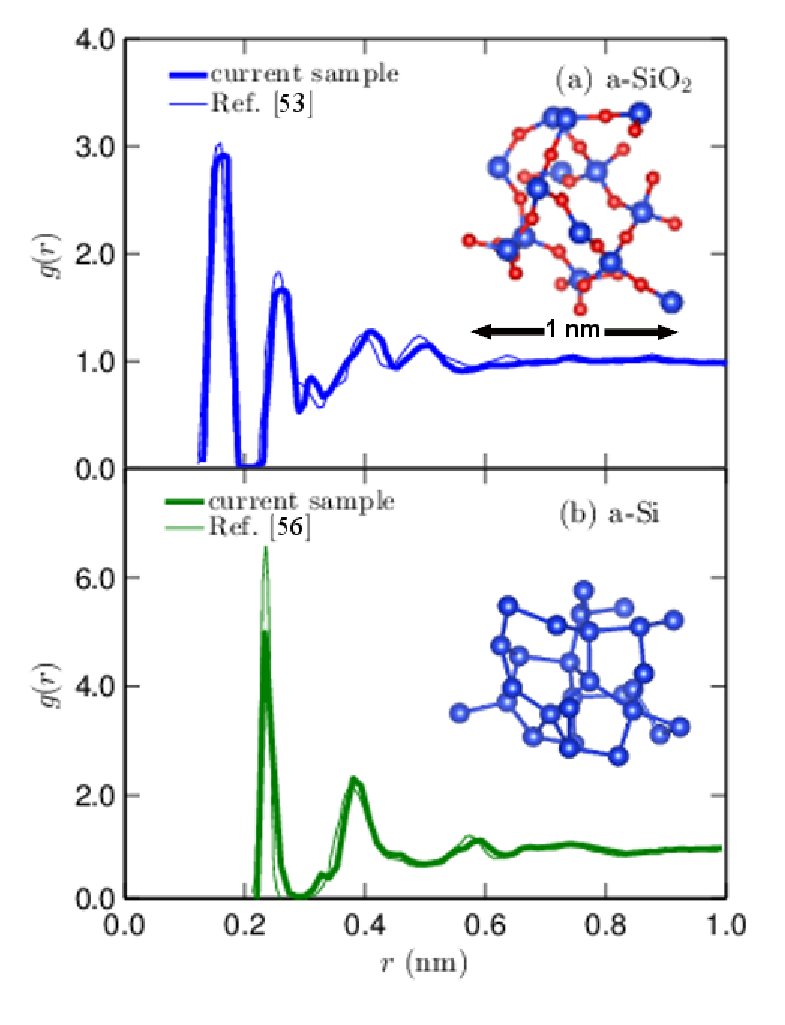
\includegraphics[scale=0.65]
{fig1.eps}
\vspace*{-5mm}
\end{center}
\caption{\label{FIG:supercell} 
\textcolor{red}{
(a) Radial distribution function, $g(r)$, for the 4608 atom a-SiO$_2$ 
structure created from a melt-quench technique. The radial distribution 
function compares well with the experimental measurement from 
Ref. \citenum{lorch_neutron_1969}. Inset: Small sample of the 
a-SiO$_2$ structure showing the Si-O tetrahedral 
bond network. Bond lengths range between 1.6 and 1.8 $\AA$.
(b) Radial distribution function for the 4096 atom a-Si 
structure created by the modified WWW 
algorithm. The radial distribution 
function compares well with the experimental measurement from 
Ref. \citenum{laaziri_high-energy_1999}. Inset: Small sample of 
the a-Si structure. Bond lengths range between 2.3 and 2.7 $\AA$. 
}
}
\end{figure}
%--------------------------------------------------------------------------
%\clearpage
\vspace{50mm}
%--------------------------------------------------------------------------
\subsection{\label{S:Simulation}Simulation Details}
%--------------------------------------------------------------------------

Before data collection, all MD simulations are first equilibrated in an 
$NVT$ (constant number of atoms, volume, and temperature) ensemble for 
$10^6$ time steps at a temperature of 300 K. Data are then collected from 
simulations in the $NVE$ (constant number of atoms, volume, and total
energy) ensemble 
for $2^{21}$ time steps, where the atomic trajectories are sampled 
every $2^{8}$ time steps. Ten MD simulations with different initial 
conditions are run and the predictions are ensemble-averaged. 

The Green-Kubo (GK) method is used to predict a thermal 
conductivity, $k_{GK}$,\cite{mcquarrie_statistical_2000} 
without using Eq. \eqref{EQ:kvib} using the 
first-avalanche method to specify the converged value of the integral 
of the heat current autocorrelation function (Section \ref{S:Bulk}).
\cite{chen_how_2010} 
For system sizes of 4608 (a-SiO$_2$, supercell side length of 4.026 nm) 
and 4096 (a-Si, supercell side length of 4.344 nm) atoms, 
the trajectories from the MD simulations are also used to predict 
the vibrational mode lifetimes using the NMD method 
(Section \ref{S:Life}). 

For an amorphous supercell, 
the only allowed wave vector is the Gamma point 
(i.e., $\pmb{\kappa}=0$),  
where $\pmb{\kappa}$ is the wavevector and there are $3N_a$ 
polarization 
branches labeled by $\nu$, where $N_a$ is the number of atoms. 
Specification of the vibrational modes at the Gamma point  
requires the eigenvalue solution of a dynamical matrix of size 
$(3N_a)^2$ that scales as $[(3N_a)^2]^3$, limiting the system 
sizes that can be considered to 4608 (a-SiO$_2$) and 4096 (a-Si) 
atoms. 
The eigenvalue solution is also required to predict the vibrational 
DOS (Section \ref{S:DOS}) and structure factors 
(Section \ref{S:Structure}), and to perform the NMD calculations  
(Section \ref{S:Life})  
and the AF calculations (Section \ref{S:Diffusivities}). 
The frequencies and eigenvectors were computed using harmonic
lattice dynamics calculations with GULP.\cite{gale_general_2003} 
The calculation of the AF thermal diffusivities 
[Eq. \eqref{EQ:DAF}] is performed using GULP and a Lorentzian 
broadening of $14\delta\omega_{avg}$ for a-SiO$_2$ and 
$5\delta\omega_{avg}$ for a-Si, 
where $\delta\omega_{avg}$ is the average mode 
frequency spacing 
[$\delta\omega_{avg} = 1.8 \times 10^{10}$ rads$/$s (a-SiO$_2$) 
and $1.0 \times 10^{10}$ rads$/$s (a-Si)].
\cite{feldman_thermal_1993,feldman_numerical_1999}  
Varying the broadening by 10$\%$ around these values does not 
change $k_{AF}$ within its uncertainty 
(Section \ref{S:Bulk}).

%--------------------------------------------------------------------------
\section{\label{S:Vibrational}Vibrational Mode Properties}
%--------------------------------------------------------------------------

%--------------------------------------------------------------------------
\subsection{\label{S:DOS}Density of States}
%--------------------------------------------------------------------------

The vibrational DOS is computed from  
\begin{equation}\label{EQ:DOS}
DOS(\omega) = \sum_i \delta(\omega_i - \omega),
\end{equation}
where a unit step function of width $100\delta\omega_{avg}$ 
is used to broaden $\delta(\omega_i - \omega)$.   
The results for a-SiO$_2$ and a-Si are plotted in Fig. \ref{FIG:DOS}. 
The DOS for a-Si is similar to that of crystalline silicon,
\cite{allen_diffusons_1999,donadio_atomistic_2009} with 
peaks at mid- and high-frequencies. The DOS for 
a-SiO$_2$ is constant over most of the frequency-range, 
with a gap that separates the high-frequency Si-O
interactions.\cite{mcgaughey_thermal_2004} 
There is a clear $\omega^{-2}$ scaling for both 
a-Si and a-SiO$_2$ at the lowest frequencies. 
The onset of this scaling occurs at a higher frequency 
for a-Si ($\sim$ 1.5 $\times 10^{13}$ rads/s) 
than a-SiO$_2$ ($\sim$ 4.5 $\times 10^{12}$ rads/s). 
This low-frequency scaling is predicted 
by the Debye model [Eq. \eqref{EQ:DOS_debye}] 
and suggests that these modes may be 
propagating (i.e., phonon-like). 

%--------------------------------------------------------------------------
\begin{figure}
\begin{center}
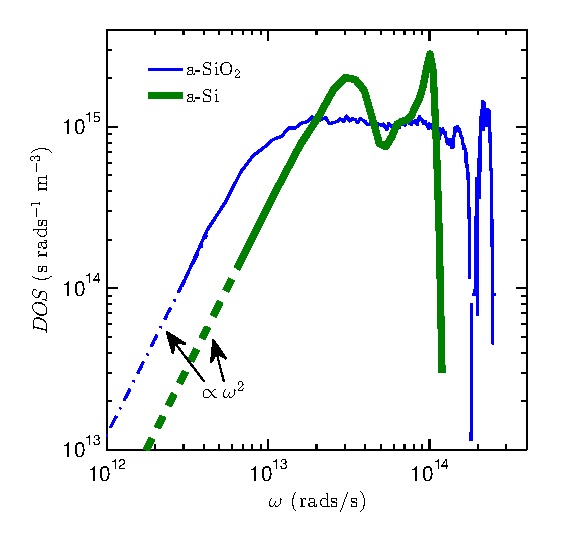
\includegraphics[scale=1.0]
{fig2.eps}
\vspace*{-5mm}
\end{center}
\caption{\label{FIG:DOS} Vibrational DOS of a-SiO$_2$ and a-Si 
plotted on a log-log scale. 
\textcolor{red}{
Both models show an $\omega^{2}$ scaling at low frequency. The 
dashed lines indicate an extrapolation of the DOS based on this scaling. 
The DOS for a-Si has two peaks similar to the 
DOS of the crystalline phase.\cite{landry_effect_2010} 
The DOS for a-SiO$_2$ is flat over most of the spectrum, with a high 
frequency gap that separates 
the modes involving Si-O interactions.\cite{mcgaughey_thermal_2004} 
}
}
\end{figure}
%--------------------------------------------------------------------------
%\clearpage
\vspace{100mm}

%--------------------------------------------------------------------------
\subsection{\label{S:Structure}Structure Factor}
%--------------------------------------------------------------------------

\textcolor{red}{
Calculating the structure factors of the 
disordered modes of the supercell at the Gamma point 
is a method to test for their propagating (i.e., plane-wave)  
character at a particular wavevector and 
polarization. 
}
This approach has been previously used to predict 
effective dispersion curves of disordered and amorphous materials 
experimentally
\cite{benassi_evidence_1996,ruocco_high-frequency_2001,
ruzicka_evidence_2004,baldi_thermal_2008,baldi_sound_2010,
baldi_emergence_2013}  
and 
numerically.
\cite{biswas_vibrational_1988,feldman_thermal_1993,
allen_diffusons_1999,feldman_numerical_1999,
taraskin_determination_1999,taraskin_propagation_2000,
horbach_high_2001,feldman_calculations_2002,
christie_vibrational_2007,
beltukov_ioffe-regel_2013,larkin_predicting_2013} 
The structure factor at a wavevector 
$\pmb{\kappa}$ is defined as\cite{allen_diffusons_1999} 
\begin{equation}\label{EQ:SLT}
S^{L,T}\kw = 
\sum_{\nu} E^{L,T}\kv
\delta (\omega-\omega\kgv),
\end{equation}
where the summation is over the Gamma modes, $E^{T}$ refers 
to the transverse polarization and is defined as
\begin{equation}\label{EQ:EL}
E^L\kv = 
\left|
\sum_{b} 
\hat{\pmb{\kappa}} \cdot e\kgvba 
\EXP{i\pmb{\kappa}\cdot\pmb{r}_0\ab{l=0}{b}} 
\right|^2
\end{equation}
and $E^{L}$ refers to the longitudinal polarization and is defined as
\begin{equation}\label{EQ:ET}
E^T\kv = 
\left|
\sum_{b} 
\hat{\pmb{\kappa}} \times e\kgvba 
\EXP{i\pmb{\kappa}\cdot\pmb{r}_0\ab{l=0}{b}} 
\right|^2.
\end{equation}
In Eqs. \eqref{EQ:EL} and \eqref{EQ:ET}, the $b$ summations are 
over the atoms in the disordered supercell, 
$\pmb{r}_0\ab{l=0}{b}$ refers to the equilibrium atomic position of 
atom $b$, $l$ labels the unit cells 
($l=0$ for the supercell), 
$\alpha$ labels the Cartesian coordinates, and 
$\hat{\pmb{\kappa}}$ is a unit vector.  
The vibrational mode shape is contained in the 
$3N_a$ components of its eigenvector, $e\kgvba$.
\cite{dove_introduction_1993}

The transverse and longitudinal structure factors are plotted in Figs. 
\ref{FIG:disp}(a) and \ref{FIG:disp}(b) for 
a-SiO$_2$ and a-Si for wavevectors along the 
[100] direction of the 
supercells. Because amorphous structures are isotropic, 
the structure factors are direction-independent. 
Mode frequencies, $\omega_0(\pmb{\kappa})$, and linewidths, 
$\Gamma(\pmb{\kappa})$, can be 
predicted by fitting each structure 
factor peak to a Lorentzian function of the form
\begin{equation}\label{EQ:Lorentzian_SLT}
\begin{split}
S^{L,T}\knw = 
\frac{C_0(\pmb{\kappa})}{[\omega_0(\pmb{\kappa})-\omega]^2+
\Gamma^2(\pmb{\kappa})},
\end{split}
\end{equation}
where $C_0(\pmb{\kappa})$ is a constant related to the DOS.
\cite{beltukov_ioffe-regel_2013} A dispersion relation is identified by 
plotting the $\omega_0(\pmb{\kappa})$ values in the middle panels of 
Figs. \ref{FIG:disp}(a) and \ref{FIG:disp}(b), 
where the error bars indicate the linewidths. 
For a-Si, Lorentzian fits to the structure factor peaks 
have coefficients of determination\cite{cowpe_temporally_2008} 
greater than 0.8 for $|\pmb{\kappa}|/\kappa_{max} \le$ 0.75 and less 
than 0.7 for $|\pmb{\kappa}|/\kappa_{max} >$ 0.75, 
where $\kappa_{max} = 2\pi/a$ and $a$ is the lattice constant 
of crystalline silicon (5.43 $\AA$).\cite{stillinger_computer_1985} 
For a-SiO$_2$, the coefficients of determination 
are greater than 0.8 for $|\pmb{\kappa}|/\kappa_{max} \le$ 0.2  
and less than 0.7 for 
larger wavevectors, where the structure factors peaks are less 
than an order of magnitude larger than the background. 
To evaluate $\kappa_{max}$ for a-SiO$_2$, we use a lattice 
constant of 4.8 $\AA$, which corresponds to the $a$-direction 
of quartz.\cite{wyckoff_crystal_1963} 

For a-Si, the extracted dispersion is 
nearly linear at small wavevectors with a slight 
decrease in slope at the largest values.
\cite{feldman_thermal_1993,feldman_numerical_1999} 
For a-SiO$_2$, the dispersion is concave-down for 
the smallest wavevectors considered, transitioning to a strong 
concave-up dispersion at intermediate wavevectors. 
For the intermediate wavevectors, 
the longitudinal dispersion for a-SiO$_2$ 
is well-described by the so-called 
``dispersion law for diffusons,'' where $\omega \propto \kappa^2$.
\cite{beltukov_ioffe-regel_2013} This large concave-up dispersion has 
been observed in experimental measurements and numerical models of 
amorphous materials
\cite{taraskin_determination_1999,horbach_high_2001,
feldman_calculations_2002,ruzicka_evidence_2004,baldi_thermal_2008} 
including a-SiO$_2$.\cite{taraskin_determination_1999,horbach_high_2001,
ruzicka_evidence_2004,baldi_thermal_2008} 
We note that at frequencies lower than $10^{12}$ rads/s, 
experimental measurements of a-SiO$_2$ recover a linear dispersion.
\cite{ruocco_high-frequency_2001,ruzicka_evidence_2004,
baldi_thermal_2008,baldi_sound_2010,baldi_emergence_2013} This frequency 
range is not accessible with the a-SiO$_2$ models studied in this work. 

The atomic structures of a-SiO$_2$ and a-Si play an important role 
in determining the differences in the low-frequency mode properties. 
The weakly-bonded network of tetrahedra in a-SiO$_2$
\cite{van_Beest_force_1990,kramer_interatomic_1991,
guissani_numerical_1996,mcgaughey_thermal_2004} results in a Debye 
scaling of the DOS that occurs at a lower frequency than in a-Si 
(Fig. \ref{FIG:DOS}), 
which is a network of strongly-bonded tetrahedra.
\cite{stillinger_computer_1985,biswas_vibrational_1988,
allen_diffusons_1999,barkema_high-quality_2000} 
The lower-frequency onset of the Debye-scaling of the DOS 
for a-SiO$_2$ leads to the strong non-linear dispersion 
seen in Fig. \ref{FIG:disp}(a). The behavior of the DOS and 
structure factors demonstrate a clear difference in the properties 
of the low-frequency modes for our models of a-SiO$_2$ and a-Si, which 
is further investigated in the following sections. 


%--------------------------------------------------------------------------
\begin{figure}
\begin{center}
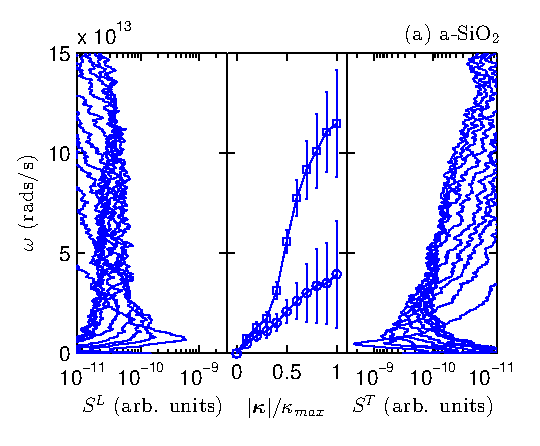
\includegraphics[scale=1.0]
{fig3b.eps}
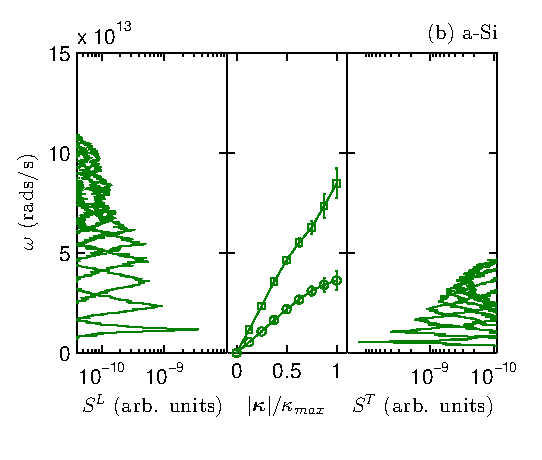
\includegraphics[scale=1.0]
{fig3a.eps}
\end{center}
\caption{\label{FIG:disp} Longitudinal (left panel) and transverse 
(right panel) structure factors [Eq. \eqref{EQ:SLT}] for (a) a-SiO$_2$ 
and (b) a-Si. 
The wavevectors are normalized by $\kappa_{max} = 2\pi/a$, where $a$ 
is 4.8 $\AA$ (a-SiO$_2$) and 5.43 $\AA$ (a-Si), based 
on the lattice constants of the crystalline phases.
\cite{wyckoff_crystal_1963,stillinger_computer_1985} }
\end{figure}
%--------------------------------------------------------------------------
%\clearpage
\vspace{130mm}

%--------------------------------------------------------------------------
\subsection{\label{S:Vg}Sound Speed}
%--------------------------------------------------------------------------

For a disordered solid,
except for the transverse and longitudinal sound speeds, there is not an
accepted method to predict the group velocity of individual 
vibrational modes.
While the structure factor gives the frequency spectrum needed to
construct a propagating state with pure wavevector $\pmb{\kappa}$,
the individual mode spectra $E^{T}\kv$ and $E^{L}\kv$ predict the
plane-wave character of each mode.
\cite{biswas_vibrational_1988,allen_diffusons_1999}
It is not generally possible
to assign a unique wavevector to individual modes, even at low frequency,
\cite{biswas_vibrational_1988,allen_diffusons_1999}
which makes predicting their group velocities challenging.
While attempts have been made to predict individual mode group velocities,
\cite{duda_reducing_2011,donadio_atomistic_2009,
he_heat_2011,he_thermal_2011,he_morphology_2011,hori_phonon_2013}
there is no theoretical basis for the proposed methods.

We now use the DOS and structure factors predicted in
Sections \ref{S:DOS} and \ref{S:Structure} to
predict the group velocities of the low-frequency modes for
a-SiO$_2$ and a-Si (i.e., the sound speeds). By fitting the DOS
from Fig. \ref{FIG:DOS} to Eq. \eqref{EQ:DOS_debye}, 
a sound speed is obtained and is 
reported in Table \ref{T:vs}. Because the DOS is a mixture of
transverse and longitudinal modes, only a single sound speed can be
predicted. 
Both longitudinal and transverse sound speeds can be predicted from
the structure factor peaks by forward differencing the dispersion relation as
\begin{equation}\label{EQ:vs_dwdk}
v_{s} = \frac{\omega_0(\kappa_{min})}{\kappa_{min}},
\end{equation}
where $\kappa_{min}$ is $0.1\kappa_{max}$ for a-SiO$_2$ and 
$0.125\kappa_{max}$ for a-Si. The results are provided in 
Table \ref{T:vs}.

The transverse and longitudinal sound speeds can
also be predicted from the material's bulk ($G$) and
shear ($K$) moduli from\cite{gale_general_2003} 
\begin{equation}\label{EQ:vs_T_elas}
v_{s,T} = \left(\frac{G}{\rho}\right)^{1/2}
\end{equation}
and
\begin{equation}\label{EQ:vs_L_elas}
v_{s,L} = \left(\frac{4G + 3K}{3\rho}\right)^{1/2}.
\end{equation}
Using the bulk and shear moduli defined in terms of the elastic
constants according to the Voight convention,\cite{gale_general_2003} 
the corresponding sound speeds are reported in Table \ref{T:vs}.
 
The longitudinal and transverse sound speeds for 
a-SiO$_2$ predicted using the moduli are 10-20\%  
lower than predictions made by Horbach et al. using a linear fit 
to the peaks of the 
current correlation function for a model with 
8016 atoms using the BKS potential 
[3568 m/s (transverse) and 5937 m/s (longitudinal)].
\cite{horbach_high_2001} The smaller 
values predicted by the structure factors and DOS 
result from the concave-down dispersion seen at low 
wavevector (i.e., we are not able to reach 
the linear portion of the dispersion curve).\cite{horbach_high_2001} 
Experimental measurements of the sound speeds of a-SiO$_2$ 
using Brillouin light and inelastic x-ray 
scattering range between 3800 to 4000 m/s (transverse) and 
6000 to 6400 m/s (longitudinal).
\cite{vacher_ultrasonic_1981,benassi_evidence_1996,
ruocco_high-frequency_2001,polian_elastic_2002,
ruzicka_evidence_2004} Differences between our predictions and 
experimental measurements may be related to limitations of the 
BKS potential.

The effect of the concave-down dispersion
is less pronounced for a-Si than for a-SiO$_2$, where the sound speeds 
predicted by all three methods are within five percent of each other. 
Our sound speed predictions for a-Si using all three methods
are within $10\%$ of predictions made using the elastic moduli
\cite{kluge_elastic_1988,feldman_elastic_1991} 
and structure factor\cite{feldman_calculations_2002} 
from models created by the original WWW algorithm.
\cite{wooten_computer_1985} 
The 4096 atom model created by the modified WWW algorithm 
\cite{barkema_high-quality_2000} predicted a longitudinal sounds 
speed of 7670 m/s from the structure factor,
\cite{christie_vibrational_2007} within $5\%$ of our prediction. 
In an attempt to explain the 
anomalously high longitudinal sound speed (8300 m/s) and 
thermal conductivity measurements in Ref. \citenum{liu_high_2009}, 
three 1000 atom a-Si models relaxed using a tight-binding electron 
structure method predicted an average of 4740 m/s (transverse) and 
7830 m/s (longitudinal).\cite{liu_high_2009} By annealing our 
structures to remove metastability, 
the sound speeds predicted by the elastic moduli are increased, but 
not by the amount reported in Ref. \citenum{liu_high_2009}. 
Experimental transverse sound speeds measurements using Rayleigh wave 
scattering are 3420 and 4290 m/s for sputtered 
and ion-bombarded a-Si thin films,\cite{vacher_attenuation_1980} which 
is within $15\%$ of the predictions from our models. 
It is clear that the experimentally-measured sound speeds for a-Si 
show a wide range, which depends on the deposition method and impurity 
concentration.
\cite{vacher_attenuation_1980,liu_high_2009,yang_anomalously_2010}

The sound speed $v_{s,DOS}$ will be used for both 
a-SiO$_2$ and a-Si for the rest of this work, allowing 
for the use of a single polarization for the propagating 
contribution [Eq. \eqref{EQ:kph}]. 
By comparing the sound speeds in Table \ref{T:vs}, it is clear that 
the low-frequency DOS of our models for a-Si and a-SiO$_2$ are 
dominated by 
transverse modes, which is expected due to their degeneracy and lower 
frequencies compared to the longitudinal modes.  
The transverse sound speed predicted for our model of 
a-SiO$_2$ is $85\%$ of that predicted by 
the other methods (Table \ref{T:vs}) and that measured by experiment.
\cite{vacher_ultrasonic_1981,benassi_evidence_1996,
ruocco_high-frequency_2001,polian_elastic_2002,
ruzicka_evidence_2004} 
While using a smaller transverse sound speed 
leads to an underprediction of the
mode diffusivities [Eq. \eqref{EQ:Dtau}], it leads to an
overprediction of the DOS [Eq. \eqref{EQ:DOS_debye}]. 
Holding all other input parameters in Eq. \eqref{EQ:kvib} constant,
a smaller sound speed leads to a larger $k_{pr}$ 
because the DOS scales as $1/v^3_{s}$. We can thus regard
our $k­_{pr}$ prediction as an upper bound.

%--------------------------------------------------------------------------
\begin{center}
\begingroup
%\squeezetable
\begin{table}
\caption{\label{T:vs}
Longitudinal and transverse sound speeds in m/s estimated from the 
elastic moduli [Eqs. \eqref{EQ:vs_T_elas} and \eqref{EQ:vs_L_elas}], 
structure factors [Eq. \eqref{EQ:vs_dwdk}], and 
DOS [Eq. \eqref{EQ:DOS_debye}]. The pre-annealed group velocities 
predicted by the elastic constants are labeled as Moduli$^*$.}
%\begin{ruledtabular}
\begin{tabular}{lllll}
\hline \hline
Method & DOS & $S^{T}, S^{L}$ & Moduli$^*$ & Moduli \\
\hline
a-SiO$_2$ \\
\hline
Transverse & 2,528 & 2,732 & 2,541 & 3,161 \\
Longitudinal &  & 4,779 & 4,761 & 5,100 \\
\hline
a-Si \\
\hline
Transverse & 3,615 & 3,699 & 3,670 & 3,886 \\
Longitudinal &  & 8,047 & 7,840 & 8,271 \\
\hline \hline
\end{tabular}
%\end{ruledtabular}
\end{table}
\endgroup
\end{center}
%--------------------------------------------------------------------------
\vspace{10mm}

%--------------------------------------------------------------------------
\subsection{\label{S:Life}Lifetimes}
%--------------------------------------------------------------------------

We now predict the lifetimes of all vibrational modes in our 
models of a-SiO$_2$ and a-Si using the MD simulation-based NMD method,
\cite{ladd_lattice_1986,mcgaughey_quantitative_2004,henry_spectral_2008,
turney_predicting_2009,
he_heat_2011,larkin_comparison_2012,hori_phonon_2013} 
which explicitly includes the disorder in the supercell.
\cite{he_heat_2011,he_thermal_2011,he_morphology_2011,
he_lattice_2012,larkin_predicting_2013} In NMD, the 
atomic trajectories from an MD simulation are first mapped onto the 
vibrational mode coordinate time derivatives,
\cite{dove_introduction_1993}
\begin{equation}\label{EQ:qdot}
\begin{split}
\dot{q}\kgvt{}{}{}=&\SUM{0}{}\sqrt{\frac{m_b}{N}}\dot{u}_{\alpha}
\lbt e^*\kgvba\EXP{i(\pmb{0}\cdot\mathbf{r}_0\ab{l}{0}}.
\end{split}
\end{equation}
Here, $m_b$ is the mass of the $b_{th}$ atom in the supercell, 
$\dot{u}_{\alpha}$ is the $\alpha$-component 
of the atomic velocity, and $t$ is time. Because the supercells 
of a-SiO$_2$ and a-Si are disordered, the NMD method can only be 
performed at the Gamma point ($\pmb{\kappa} = \pmb{0}$). 
The spectral energy of each vibrational mode, $\Phi(\nu,\omega)$, 
is calculated from 
\begin{equation}\label{A:E:Phi_NMD}
\begin{split}
\Phi(\nu,\omega) = 
\lim_{\tau_0\rightarrow\infty}\frac{1}{2\tau_0}
\left|\frac{1}{\sqrt{2\pi}}\int_{0}^{\tau_0}\dot{q}\kgvt
\exp(-i\omega t)dt\right|^2.
\end{split}
\end{equation}
We choose the frequency-domain representation of the normal mode 
energy because we find it to be less sensitive to any remaining 
metastability of the amorphous structure than the time-domain 
representation. 

The vibrational mode frequency and lifetime are predicted by fitting 
each mode's spectral energy to a Lorentzian function, 
\begin{equation}\label{EQ:Lorentzian_NMD}
\begin{split}
\Phi(\nu,\omega) = 
\frac{C_0(\nu)}{[\omega_0(\nu)-\omega]^2+\Gamma^2(\nu)},
\end{split}
\end{equation}
where the constant $C_0(\nu)$ is related to the average energy of 
each mode. This expression is valid when the linewidth  
$\Gamma(\nu) << \omega_0(\nu)$.\cite{larkin_comparison_2012} 
The mode lifetime is\cite{ladd_lattice_1986,turney_predicting_2009} 
\begin{equation}\label{EQ:NMD_life}
\begin{split}
\tau(\nu) = \frac{1}{2\Gamma(\nu)}.
\end{split}
\end{equation}

The NMD-predicted lifetimes are plotted in Figs. 
\ref{FIG:Lifetimes}(a) and \ref{FIG:Lifetimes}(b) 
for a-SiO$_2$ and a-Si. 
Also plotted are the timescales extracted from the structure 
factor linewidths, $1/[2\Gamma(\kappa)]$ (Section \ref{S:Structure}). 
For a-SiO$_2$, the NMD lifetimes are larger than 
the Ioffe-Regel (IR) limit $\tau = 2\pi/\omega$,
\cite{taraskin_determination_1999} and are bounded by  
this limit at low frequencies. Similarly for a-Si, the IR limit is 
a lower limit for the lifetimes predicted by NMD. 
\textcolor{red}{
While lifetimes 
predicted near the IR limit do not satisfy the constraint 
$\Gamma(\nu) << \omega_0(\nu)$, only a limited number of these 
lifetimes are used to determine the coefficient of the low-frequency 
scaling [see Figs. \ref{FIG:diffusivities} (a) and (b)]. 
}

There is no clear evidence for an $\omega^{-2}$ scaling in a-SiO$_2$, 
which would correspond to propagating modes.  
At mid-frequencies, the NMD lifetimes are approximately constant and  
there is a peak near 2 $\times 10^{14}$ rads$/$s, which corresponds to 
the peak in the DOS (see Fig. \ref{FIG:DOS}). 
The timescales predicted from the 
structure factor fall below the NMD-predicted lifetimes 
and the IR limit by up to one order of magnitude. 
These low values result because the structure factors 
for a-SiO$_2$ are evaluated for wavevectors where the resulting 
wavepackets are formed by non-propagating modes.
\cite{feldman_thermal_1993,feldman_numerical_1999,allen_diffusons_1999}

For a-Si, the NMD lifetimes show a clear $\omega^{-2}$ 
scaling at low frequency. 
The lifetimes plateau at higher frequencies,
over a wider range of frequencies than for a-SiO$_2$, with two peaks 
corresponding to the peaks in the DOS (see Fig. \ref{FIG:DOS}). 
A similar plateau of lifetimes at high frequencies has been 
reported for disordered lattices
\cite{sheng_heat_1991,he_lattice_2012,larkin_predicting_2013} and in 
another study of a-Si.\cite{he_heat_2011} 
The transition from the low-frequency scaling to 
the plateau region occurs near 
$10^{13}$ rads$/$s, which corresponds to where the DOS first peaks 
in Fig. \ref{FIG:DOS}. 
Similar behavior has been observed for models of disordered lattices.
\cite{larkin_predicting_2013} The timescales predicted by the 
structure factors are in good agreement with those predicted by NMD 
at low frequencies. Similar agreement has been reported in other 
models of amorphous materials.
\cite{mazzacurati_low-frequency_1996,bickham_calculation_1998,
bickham_numerical_1999,feldman_numerical_1999} 
The agreement between the 
NMD-predicted lifetimes and the structure factor timescales for a-Si 
at low frequencies indicates that these modes are plane-wave-like 
and that the wavepackets formed by these modes are propagating.
\cite{feldman_thermal_1993,feldman_numerical_1999,allen_diffusons_1999}

The NMD-predicted lifetimes for a-Si range from 0.5 to 10 ps 
and are similar in magnitude to 
those predicted for previous WWW-generated models of a-Si.
\cite{fabian_anharmonic_1996,bickham_calculation_1998,
bickham_numerical_1999,fabian_numerical_2003}  
We note that one previous study of a-Si modeled using the 
Tersoff potential predicted vibrational lifetimes on 
the order of 100 ps,\cite{he_heat_2011} an order of magnitude larger 
than the values reported here and in previous studies.
\cite{fabian_anharmonic_1996,bickham_calculation_1998,
bickham_numerical_1999,fabian_numerical_2003} 
It is unclear what the source of this 
discrepancy is, although in Ref. \citenum{he_heat_2011} 
the NMD analysis was performed in the time domain, where the effects of 
metastability can be more strongly pronounced. Using the Tersoff 
potential on the WWW a-Si models in this work, we predict similar 
lifetimes to those from the SW potential. 

%--------------------------------------------------------------------------
\begin{figure}
\begin{center}
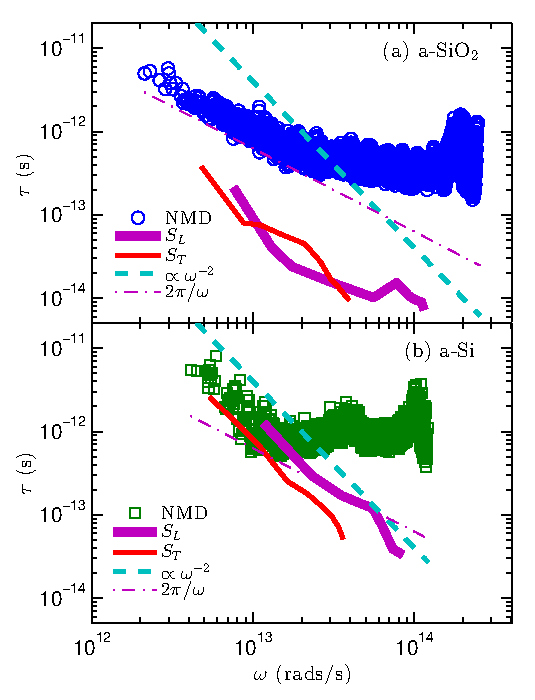
\includegraphics[scale=1.0]
{fig4.eps}
\vspace*{-5mm}
\end{center}
\caption{\label{FIG:Lifetimes} Vibrational mode lifetimes predicted by 
NMD [Eq. \eqref{EQ:NMD_life}] and the timescales extracted from the 
structure factors 
[Eq. \eqref{EQ:Lorentzian_SLT}] for (a) a-SiO$_2$ and (b) a-Si. 
For a-Si, a clear $\omega^{-2}$ scaling is observed at low frequencies, 
while the lifetimes plateau at higher frequencies and 
over a wider range of frequencies than for a-SiO$_2$.}
\end{figure}
%--------------------------------------------------------------------------
\vspace{10mm}
%\clearpage
%--------------------------------------------------------------------
%\begin{figure}
%\begin{center}
%\includegraphics[scale=1.0]
%{/home/jason/disorder/si/amor/m_si_amor_life_he_compare.eps}
%\vspace*{-5mm}
%\end{center}
%\caption{\label{FIG:phonon_diff} film thickness dependant thermal 
%conductivity of a-Si from experiment.}
%\end{figure}
%--------------------------------------------------------------------------

%--------------------------------------------------------------------------
\subsection{\label{S:Diffusivities}Diffusivities}
%--------------------------------------------------------------------------

Using the sound speeds predicted 
from the DOS (Table \ref{T:vs}), the NMD-predicted lifetimes 
for a-SiO$_2$ and a-Si are used to predict the mode diffusivities with 
Eq. \eqref{EQ:Dtau}. The results are plotted in 
Figs. \ref{FIG:diffusivities}(a) and \ref{FIG:diffusivities}(b).  
\textcolor{red}{
The mode diffusivities are predicted from the NMD lifetimes for the 
low-frequency modes where the DOS scales as $\omega^2$ 
(Fig. \ref{FIG:DOS}). The AF theory is used to predict the mode 
diffusivities for all frequencies and the results are also plotted in 
Figs. \ref{FIG:diffusivities}(a) and \ref{FIG:diffusivities}(b). 
}

For a-SiO$_2$, the mode diffusivities predicted by NMD and AF agree 
well at low frequency. The AF diffusivities at 
the highest frequencies show a sharp decrease, which is an indication 
that these modes are localized.\cite{feldman_thermal_1993} 
The low- and mid-frequency diffusivities are above the 
high-scatter limit, 
\begin{equation}\label{EQ:D_HS}
D_{HS} = \frac{1}{3} v_s a,
\end{equation}
which assumes that all vibrational modes travel with the sound speed  
and scatter over a distance of the lattice constant.
\cite{cahill_lattice_1988} In evaluating Eq. \eqref{EQ:D_HS}, 
we use the lattice constant of the 
crystalline phase (see Section \ref{S:Structure}). The low-frequency 
NMD diffusivities do not show a 
definitive scaling. Based on the results in 
Ref. \citenum{baldi_thermal_2008}, we choose a 
propagating/non-propagating cutoff frequency of 
$4.55\times10^{12}$ rads/s, which is at the onset 
of the Debye scaling of the DOS (Fig. \ref{FIG:DOS}). 
The constant $B$ in Eq. \eqref{EQ:tauw2} for $n=2$ 
is then fit to the AF-predicted diffusivities for 
frequencies below the cutoff by dividing the diffusivities 
by $v_{s,DOS}$. The fit value is $B=5.65\times10^{13}$ 
rads$^2$s$^{-1}$.

For a-Si, the mode diffusivities predicted by NMD 
show a clear $\omega^{-2}$ scaling. 
The NMD-predicted diffusivities are larger and show less 
scatter than those predicted by the AF theory, which is due to 
the finite-size system and the broadening that is 
required to evaluate 
Eq. \eqref{EQ:DAF}.\cite{feldman_thermal_1993} By using a larger 
broadening ($100\delta\omega_{avg}$), the scatter 
in the AF-predicted 
diffusivities at low frequency can be smoothed, but at the cost of 
decreasing the diffusivities at intermediate and 
high frequencies, which 
affects the predicted diffuson contribution to thermal 
conductivity (see Section \ref{S:Bulk}). 
It is possible that a frequency-dependent broadening may be 
necessary for a-Si and the AF theory,  
but determining this dependence is not necessary for 
interpreting our results. 
For a-Si, the AF diffusivities are 
larger than the high-scatter limit [Eq. \eqref{EQ:D_HS}], 
except for the highest frequency modes, which are localized.
\cite{feldman_thermal_1993} 

For a-Si, we choose $\omega_{cut}$  
and $B$ so that Eq. \eqref{EQ:Dtau} is equal 
to the average AF-predicted diffusivity at the cutoff frequency. 
The resulting values are 
$\omega_{cut}=1.16 \times 10^{13}$ rads$/$s (which is at the onset 
of the Debye scaling of the DOS, Fig. \ref{FIG:DOS})  
and $B=2.76\times10^{14}$ rads$^2$s$^{-1}$. This choice 
allows Eq. \eqref{EQ:Dtau} to pass reasonably well through both 
the AF- and NMD-predicted diffusivities. 

While experiments on a-SiO$_2$ show that there is a cross-over 
region for the low-frequency lifetime scaling from $\omega^{-2}$ to 
$\omega^{-4}$,\cite{masciovecchio_evidence_2006} 
and then back to $\omega^{-2}$,
\cite{masciovecchio_evidence_2006,baldi_sound_2010,
baldi_elastic_2011,baldi_emergence_2013} our present model is not 
large enough to investigate the mode properties 
in this cross-over region. 
Because experiments are limited for a-Si thin films, 
\cite{hondongwa_ultrasonic_2011} 
we also consider a $\omega^{-4}$ scaling 
for Eq. \eqref{EQ:tauw2}. Because this scaling is not clear from 
the data in Fig. \ref{FIG:diffusivities}(b),  
we use a cutoff frequency of 1.52 $\times 10^{13}$ rads$/$s 
(which is at the onset 
of the Debye scaling of the DOS, Fig. \ref{FIG:DOS}) 
based on Refs. \citenum{feldman_thermal_1993} and 
\citenum{cahill_thermal_1994} 
and choose $B=2.07\times10^{40}$ rads$^4$s$^{-3}$ so that 
Eq. \eqref{EQ:Dtau} is equal to the average 
AF-predicted diffusivity at the cutoff frequency. 

Both a-SiO$_2$ and a-Si have a region at higher frequencies where 
the AF-predicted mode diffusivities are relatively constant. This 
behavior has been reported for model disordered systems such as 
disordered lattices\cite{sheng_heat_1991,beltukov_ioffe-regel_2013,
larkin_predicting_2013} and jammed systems.
\cite{xu_energy_2009,vitelli_heat_2010}  
While diffusons are non-propagating modes whose MFPs are not 
well-defined,\cite{feldman_thermal_1993} 
a diffuson MFP can be calculated from 
\begin{equation}\label{EQ:LambdaAF}
\begin{split}
\Lambda_{AF}(\omega_i) = [3D_{AF}(\omega_i)\tau(\omega_i)]^{1/2},
\end{split}
\end{equation}
where $\tau(\omega_{i})$ is the NMD-predicted lifetime for that mode. 
Using this definition, $\Lambda_{AF}(\omega_i)$ for both a-SiO$_2$ 
and a-Si is found to vary between the crystal lattice constant 
($\sim 0.5$ nm) and 
the supercell size ($\sim 5$ nm) 
for modes with frequency above the cutoff. 
Similar MFPs have been estimated for diffusons in a-Si in 
previous studies.\cite{feldman_thermal_1993,feldman_numerical_1999} 
For modes with frequency below the cutoff, the NMD-predicted 
MFPs from Eq. \eqref{EQ:Lambda} range up to 16 nm (a-SiO$_2$) 
and 43 nm (a-Si). This result is in contrast to the MFPs 
estimated in Ref. \citenum{he_heat_2011} for a-Si, which ranged 
up to 500 nm. We believe that the origin of the large MFPs 
in Ref. \citenum{he_heat_2011} is 
a combination of the predicted lifetimes (see Section \ref{S:Life}) 
and the method used to estimate the mode group velocities.

%--------------------------------------------------------------------------
\begin{figure}
\begin{center}
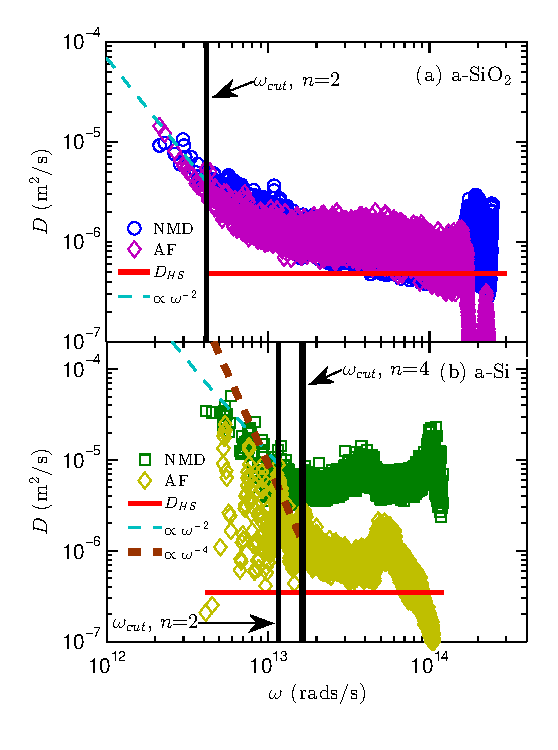
\includegraphics[scale=1.0]
{fig5.eps}
\vspace*{-5mm}
\end{center}
\caption{\label{FIG:diffusivities} Vibrational mode diffusivities 
predicted from NMD [using Eqs. \eqref{EQ:Dtau} and 
\eqref{EQ:NMD_life} with the DOS sound speed from Table \ref{T:vs}] 
and the AF theory [Eq. \eqref{EQ:DAF}]. 
Also shown are  
extrapolations based on an $\omega^{-2}$ scaling with 
Eqs. \eqref{EQ:Dtau} and \eqref{EQ:tauw2} for a-SiO$_2$ and a-Si, 
and an additional $\omega^{-4}$ scaling for a-Si. For both systems, 
the diffusivities are larger than the high-scatter limit 
[Eq. \eqref{EQ:D_HS}] except at high frequencies, where the modes 
are localized.
}
\end{figure}
%--------------------------------------------------------------------------
\vspace{20mm}
%\clearpage

%--------------------------------------------------------------------------
% \begin{figure}
% \begin{center}
% \includegraphics[scale=1.0]
% {/home/jason/disorder/si/amor/m_af_si_normand_4096_vAF.eps}
% \vspace*{-5mm}
% \end{center}
% \caption{\label{FIG:Lifetimes} .}
% \end{figure}
%--------------------------------------------------------------------------

%\clearpage
%\vspace{50mm}

% %--------------------------------------------------------------------------
% \begin{figure}
% \begin{center}
% \includegraphics[scale=1.0]
% {/home/jason/disorder/si/amor/m_af_si_normand_4096_Lambda_3.eps}
% \vspace*{-5mm}
% \end{center}
% \caption{\label{FIG:mfp} vibrational MFPs predicted from NMD using Eq. 
% \eqref{EQ:Lambda} and the sound speed predicted in Table \ref{T:vs}
% and from NMD and AF using Eq. \eqref{EQ:LambdaAF}. Good agreement 
% between the two methods is seen at low frequency, indicating that the 
% modes are propagating and Eqs. \eqref{EQ:Dtau} and \eqref{EQ:DLambda} 
% are valid. The majority of MFPs in the intermediate the high-frequency range 
% lie between the simulation box size $L$ and the bond distance $a$. The 
% inset compares the representative mode velocities Eq. \eqref{EQ:vAF} and 
% the sound speeds. For a-Si, $v_{AF}$ decreases with increasing frequency, 
% similar to the behavior of a monatomic crystal.(cite) The MFPs and 
% mode velocities only approach zero at the highest frequencies, which is 
% an indication that the modes are localized.}
% \end{figure}
% %--------------------------------------------------------------------------

%\clearpage
%\vspace{50mm}

%--------------------------------------------------------------------------
\section{\label{S:Conductivity}Thermal Conductivity}
%--------------------------------------------------------------------------

%--------------------------------------------------------------------------
\subsection{\label{S:Bulk}Bulk}
%--------------------------------------------------------------------------

To predict the bulk thermal conductivity for our models of a-SiO$_2$ and 
a-Si, we use both Eq. \eqref{EQ:kvib} and the GK method. The GK method 
is computationally inexpensive compared to the NMD and AF methods so that 
larger system sizes can be accessed. The GK-predicted thermal 
conductivities for a-SiO$_2$ and a-Si are plotted in Fig. \ref{FIG:cond} 
versus the inverse of the length of the simulation cell. For a-SiO$_2$, 
there is no system-size dependence.  The bulk thermal conductivity is 
estimated to be $2.1 \pm 0.2$ W/m-K by averaging over all the samples. 
This prediction is in agreement with the GK predictions in Ref. 
\citenum{mcgaughey_thermal_2004} within the uncertainties, 
but larger than the MD-based direct-method predictions in Ref. 
\citenum{jund_molecular-dynamics_1999}. 
Shenogin et al. predicted the total thermal 
conductivity of a-SiO$_2$ using 
non-equilibrium MD simulations of the same small structures 
used in this work. They find 2.0 W/m-K for their 
largest system, which was based on a 972 atom model 
tiled six times in one direction.\cite{shenogin_predicting_2009}
Our GK-predicted value is larger than experimental 
measurements, which range between 
1.3 and 1.5 W/m-K,
\cite{cahill_lattice_1988,lee_heat_1997,
yamane_measurement_2002,regner_broadband_2013} 
which may be due to the classical nature of the MD simulation 
and/or the suitability of the BKS interatomic potential 
for modeling thermal transport in a-SiO$_2$.
\cite{jund_molecular-dynamics_1999,mcgaughey_thermal_2004}
Quantum statistical effects are considered later in this section. 

For a-Si, there is a clear system-size dependence of thermal 
conductivity. 
Because the low-frequency DOS has the form of Eq. \eqref{EQ:DOS_debye} 
and the diffusivities scale as $\omega^{-2}$,  
the thermal conductivity will scale as the inverse of the system size. 
The bulk value can be found by extrapolating to an infinite system size.
\cite{shiomi_thermal_2011,esfarjani_heat_2011,larkin_comparison_2012} 
The extrapolation is performed using the three largest 
system sizes,\cite{mfp_fn2} leading to a bulk value 
of $2.0 \pm 0.2$ W/m-K, where the uncertainty is 
estimated from the ensemble averaging for each system size. 
Our extrapolated bulk value 
is in reasonable agreement with experimental values for a wide 
range of thin film thicknesses (see Fig. \ref{FIG:sio2_accum} in 
Section \ref{S:Accumulation}). 
\textcolor{red}{
We note that a-Si can be only prepared experimentally as a thin film, 
where voids and other inhomogeneities are unavoidable
\cite{vacher_attenuation_1980,feldman_thermal_1993,liu_high_2009,
yang_anomalously_2010,li_effect_2011} and can influence the 
vibrational structure at low frequencies.
\cite{feldman_tight-binding_2004,liu_high_2009}
}

To predict thermal conductivity from Eq. \eqref{EQ:kvib}, 
we use the parameters $B$ and $\omega_{cut}$ specified 
in Section \ref{S:Diffusivities} assuming an $\omega^{-2}$ 
scaling below $\omega_{cut}$ and the AF-predicted diffusivities. 
For a-SiO$_2$, the propagating, non-propagating, and total thermal 
conductivities are 0.10 $\pm$ 0.05, 1.9 $\pm$ 0.1, 
and 2.0 $\pm$ 0.1 W/m-K (see Table \ref{T:cond}). The uncertainties 
are estimated by varying $\omega_{cut}$ and the AF 
broadening by $10\%$.  
The total value agrees with the GK value within the uncertainties. 
For the propagating contribution, 
using an expression similar to Eq. \eqref{EQ:kph}, 
Baldi et al.\cite{baldi_thermal_2008} estimated $0.1$ W/m-K and 
Love and Anderson\cite{love_estimate_1990} estimated 0.03 W/m-K.
% Their predicted non-propagating conductivities are smaller than 
% those in this work, which is due to a smaller broadening used for 
% Eq. \eqref{EQ:DAF}.  

By using the $\omega^{-2}$ diffusivity scaling for a-Si, 
the propagating, non-propagating, and total thermal conductivities 
are 0.6 $\pm$ 0.1, 1.2 $\pm$ 0.1, and 1.8 $\pm$ 0.2 W/m-K. 
This value for total thermal conductivity 
is in agreement with the GK-predicted bulk value within the 
uncertainties. Earlier studies using 
similar models of a-Si found 
that $k_{pr}$ is less than half of 
$k_{vib}$,\cite{feldman_thermal_1993,
feldman_numerical_1999} in agreement with our results.  
A recent study of a-Si modeled using the Tersoff potential found 
$k_{pr} \approx k_{AF}$.\cite{he_heat_2011} 
Estimates based on experimental measurements 
have found $k_{pr}$ to be as low 
as $~20\%$\cite{cahill_thermal_1994,feldman_numerical_1999} 
and as high as $~80\%$ of $k_{vib}$.
\cite{liu_high_2009,yang_anomalously_2010}

If an $\omega^{-4}$ lifetime scaling is assumed for a-Si, 
the thermal conductivity diverges at low frequency. We bound the 
thermal conductivity by assuming the sample to be a thin film 
of thickness $t_f$ and modify the lifetimes using the Matthiessen 
rule,\cite{ziman_electrons_2001} 
\begin{equation}\label{EQ:LambdaMatth}
\begin{split}
\frac{1}{\tau_{eff}} = \frac{1}{\tau_{bulk}} + 
\frac{2v_s}{t_f}.
\end{split}
\end{equation}
Using the largest film thickness from the experimental 
literature ($80$ $\mu$m)\cite{liu_high_2009} 
gives a propagating contribution 
to thermal conductivity of $3.0 \pm 0.4$ W/m-K, which is 
significantly larger than GK-predicted value. 
Using the $\omega^{-2}$ scaling and this film thickness 
gives a propagating contribution of 0.6 W/m-K (i.e., there is 
no change from the bulk value). 
While predictions for $k_{pr}$ for a-Si  
vary based on the assumed scaling of the low-frequency 
vibrational lifetimes
\cite{feldman_thermal_1993,cahill_thermal_1994,
feldman_numerical_1999,liu_high_2009,yang_anomalously_2010,
he_heat_2011} 
all evidence supports that $k_{pr}$ is a significant fraction 
of the total thermal conductivity.
\cite{feldman_thermal_1993,cahill_thermal_1994,
feldman_numerical_1999,liu_high_2009,
yang_anomalously_2010,
he_heat_2011,regner_broadband_2013}

To this point we approximated the specific heat 
of the propagating 
and non-propagating modes by the classical, harmonic-limit 
value of $k_{\text{B}}$. At a temperature of $300$ K, the quantum 
heat capacity [Eq. \eqref{EQ:Cquantum}] 
at the largest cutoff frequency for either a-SiO$_2$ or a-Si 
is $0.98 k_{\text{B}}$, justifying the 
use of the classical specific heat in the propagating term 
in Eq. \eqref{EQ:kph}. For the AF contribution, however, the 
effect of the quantum specific heat is important. At the highest 
frequency in each of a-SiO$_2$ and a-Si, the specific heat is 
0.073$k_{\text{B}}$ and 0.47$k_{\text{B}}$. 
Using Eq. \eqref{EQ:Cquantum} 
in Eq. \eqref{EQ:kAF} gives AF thermal conductivities of 
1.4 $\pm$ 0.1 and 
1.0 $\pm$ 0.1 W/m-K for a-SiO$_2$ and a-Si (Table \ref{T:cond}). 
This correction brings the estimate of $k_{vib}$ for 
a-SiO$_2$ into good agreement with experimental measurements.
\cite{cahill_lattice_1988,lee_heat_1997,
yamane_measurement_2002,regner_broadband_2013} 
For a-Si, the modified $k_{AF}$ is 20$\%$ lower than the 
classical-limit value. 

%--------------------------------------------------------------------------
\begin{figure}
\begin{center}
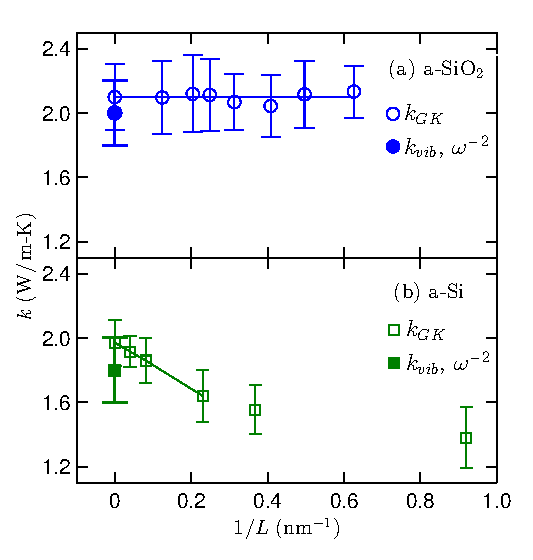
\includegraphics[scale=1.0]
{fig6.eps}
\vspace*{-5mm}
\end{center}
\caption{\label{FIG:cond} Thermal conductivities of a-SiO$_2$ and 
a-Si predicted using the GK method and Eq. \eqref{EQ:kvib}. 
For a-SiO$_2$, the GK-predicted thermal conductivity 
is size-independent, indicating that there is not an important 
contribution from propagating modes. For a-Si, there is a clear size 
dependance, indicating the importance of propagating modes. }
\end{figure}
%--------------------------------------------------------------------------
%\clearpage
\vspace{100mm}
%--------------------------------------------------------------------------
\begin{center}
\begingroup
\squeezetable
\begin{table}
\caption{\label{T:cond}
Thermal conductivities for bulk a-SiO$_2$ and a-Si 
predicted by the GK method ($k_{GK}$) and 
Eqs. \eqref{EQ:kvib} ($k_{vib}$), \eqref{EQ:kph} ($k_{pr}$), and 
\eqref{EQ:kAF} ($k_{AF}$). 
For the non-propagating contribution, classical and quantum 
specific heats are considered. 
}
%\begin{ruledtabular}
\begin{tabular}{llllll}
\hline\hline
Thermal Conductivity (W/m-K) & a-SiO$_2$ & a-Si & \\
\hline
$k_{GK}$ & 2.1 $\pm$ 0.2 & 2.0 $\pm$ 0.2 & \\
$k_{vib}$ (classical) & 2.0 $\pm$ 0.1 & 1.8 $\pm$ 0.2 & \\
$k_{pr}$ & 0.10 $\pm$ 0.05 & 0.6 $\pm$ 0.2 & \\
$k_{AF}$ (classical) & 1.9 $\pm$ 0.1 & 1.2 $\pm$ 0.1 & \\
$k_{AF}$ (quantum) & 1.4 $\pm$ 0.1 & 1.0 $\pm$ 0.1 & \\
$k_{vib}$ (quantum) & 1.5 $\pm$ 0.1 & 1.6 $\pm$ 0.2 & \\
\hline\hline
\end{tabular}
%\end{ruledtabular}
\end{table}
\endgroup
\end{center}
%--------------------------------------------------------------------------
%\clearpage
\vspace{200mm}


% \begin{center}
% \begin{table}
% \begin{tabular}{llllll}
% \hline\hline
% $\phi$ & $L_{eq}$& $k$ (Matthiessen Rule w/$L_{eq}$)& $k$(Free Path Sampling)\\
% & (nm) & (W/m-K) & (W/m-K) \\
% \hline
% $0.1$ & $405$ & $91$ & $84$\\
% $0.2$ & $365$ & $89$ & $78$\\
% $0.3$ & $275$ & $85$ & $72$\\
% $0.4$ & $270$ & $85$ & $67$\\
% $0.5$ & $225$ & $82$ & $62$\\
% \hline\hline
% \end{tabular}
% \end{table}
% \end{center}

%--------------------------------------------------------------------------
\subsection{\label{S:Accumulation}Accumulation Function}
%--------------------------------------------------------------------------

In their broadband frequency domain thermoreflectance 
measurements, Regner et al.,\cite{regner_broadband_2013}  
adopting the convention of Koh and Cahill,\cite{koh_frequency_2007} 
interpret the  
measured thermal conductivity at a given thermal penetration depth 
to be representative of the thermal conductivity accumulation 
function at a MFP equal to the thermal penetration depth.
\cite{dames_thermal_2005,yang_mean_2013} 
Their results are plotted in Fig. \ref{FIG:sio2_accum}(a) 
for a 1000 nm thick film of a-SiO$_2$ 
and in Fig. \ref{FIG:sio2_accum}(b) for 500 nm and 
2000 nm thick films of a-Si. The vertical coordinate 
of any point on the accumulation function represents the thermal 
conductivity that comes from phonons with MFPs less than the 
horizontal coordinate at that point. Also plotted in 
Figs. \ref{FIG:sio2_accum}(a) and \ref{FIG:sio2_accum}(b) 
are experimental measurements of thin film thermal 
conductivities. For a-Si, the experimental measurements are 
broadly grouped by sample preparation technique: 
(A) chemical vapor deposition
\cite{moon_thermal_2002,liu_high_2009,yang_anomalously_2010}
and (B) sputtering.
\cite{kuo_thermal_1992,cahill_thermal_1994,wada_thermal_1996} 

Based on the results in Section \ref{S:Diffusivities}, we build 
thermal conductivity accumulation functions for a-SiO$_2$ and a-Si 
from
\begin{equation}\label{EQ:kLambda}
k(\Lambda^{*}) = k_{AF} + 
\int^{\Lambda^{*}}_{\Lambda_{cut}} 
k(\Lambda)d\Lambda,
\end{equation}
where $\Lambda_{cut}$ is the MFP at the cut-off frequency, 
$\Lambda^*$ is the maximum MFP considered in the thermal 
conductivity accumulation, $k(\Lambda)$ is the thermal conductivity 
as a function of MFP,\cite{yang_mean_2013} 
and the propagating mode MFPs are 
calculated using lifetimes from Eq. \eqref{EQ:LambdaMatth}. The 
non-propagating contribution $k_{AF}$ is evaluated using the quantum 
specific heat (see Section \ref{S:Bulk}). 
The results are plotted for a-SiO$_2$ 
in Fig. \ref{FIG:sio2_accum}(a) using an infinite film thickness 
and for a-Si in Fig. \ref{FIG:sio2_accum}(b) using a film 
thickness of $80$ $\mu$m.\cite{mfp_fn3}  

The predicted thermal conductivity accumulation function for a-SiO$_2$ 
saturates at a MFP of 10 nm, which is on the order of the finite size 
of our model. This result is in good quantitative agreement 
with the thermal penetration depth-independent thermal 
conductivity measurements using broadband frequency domain 
thermoreflectance\cite{regner_broadband_2013} and experimental 
measurements that show minimal film-thickness dependance.
\cite{lee_heat_1997,yamane_measurement_2002} 

For a-Si, the low-MFP plateau of thermal conductivity in the   
measurements of Regner et al. is consistent with our 
predicted $k_{AF}$. 
The propagating contribution to the accumulation is predicted 
using $\omega^{-2}$ and $\omega^{-4}$ lifetime scalings, which 
have both been inferred from thin film experiments.
\cite{feldman_thermal_1993,cahill_thermal_1994,
feldman_numerical_1999,zink_thermal_2006,zink_excess_2006,
liu_high_2009,yang_anomalously_2010} 
Predictions for both the $\omega^{-2}$ and $\omega^{-4}$ scalings 
pass reasonably through the thin film thermal conductivity 
measurements, particularly for thicknesses in the 50-2000 nm range. 
Overall, the film-thickness dependent measurements show a large 
variation which results from the deposition method and impurity 
concentration.
\cite{vacher_attenuation_1980,liu_high_2009,yang_anomalously_2010,
li_effect_2011} 
The measurements of Regner et al. show sharper accumulations 
than either the $\omega^{-2}$ or $\omega^{-4}$ scalings, 
particularly for the $2000$ nm film. 
For the $\omega^{-2}$ scaling, which best matches our model 
[see Fig. \ref{FIG:Lifetimes}(b)], 
the thermal conductivity accumulation 
saturates at $1$ $\mu$m, in good agreement with where the measurements 
of Regner et al. saturate for their 500 nm film. The 2000 nm 
film accumulation shows no sign of saturation. 


%--------------------------------------------------------------------------
% \begin{figure}
% \begin{center}
% \includegraphics[scale=1.0]
% {/home/jason/disorder/si/amor/m_af_si_normand_4096_kLamba_6_sio2.eps}
% \vspace*{-5mm}
% \end{center}
% \caption{\label{FIG:si_accum} Predicted thermal conductivity 
% accumulation function [Eq. \eqref{EQ:kLambda} 
% for a-SiO$_2$ compared with experimental measurements 
% by Regner et al.,\cite{regner_broadband_2013} 
% Love and Anderson (Expt. A),\cite{love_estimate_1990} 
% and Yamane et al. (Expt. B).\cite{yamane_measurement_2002}
% The predicted thermal conductivity accumulation demonstrates that 
% the propagating contribution is negligible in our model, which is 
% in accord with the experimental measurements.
% }
% \end{figure}
%--------------------------------------------------------------------------

%--------------------------------------------------------------------------
\begin{figure}
\begin{center}
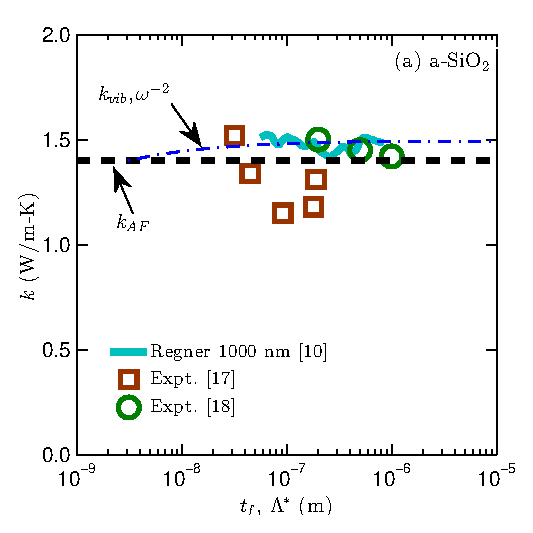
\includegraphics[scale=1.0]
{fig7a.eps}
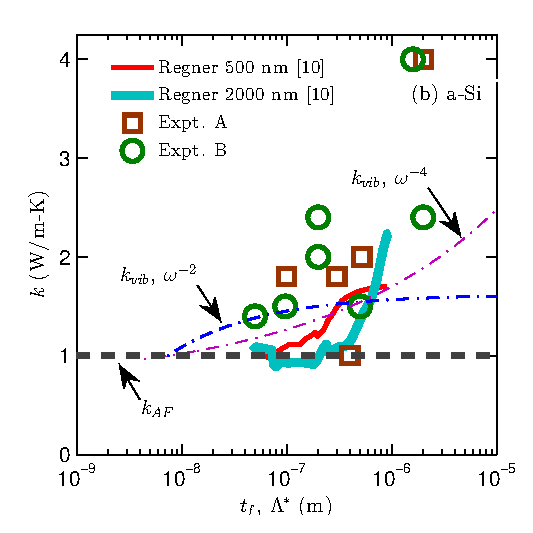
\includegraphics[scale=1.0]
{fig7b.eps}
\vspace*{-5mm}
\end{center}
\caption{\label{FIG:sio2_accum} 
{\scriptsize
(a) Predicted thermal conductivity 
accumulation function [Eq. \eqref{EQ:kLambda}]  
for a-SiO$_2$ compared with experimental broadband frequency 
domain reflectance measurements 
by Regner et al.\cite{regner_broadband_2013} and thin film 
measurements from Refs. \citenum{lee_heat_1997} and 
\citenum{yamane_measurement_2002}. 
The predicted thermal conductivity accumulation demonstrates that 
the propagating contribution is negligible in our model, which is 
in accord with the experimental measurements. 
(b) Predicted thermal conductivity 
accumulation function 
for a-Si compared with experimental measurements 
by Regner et al. and thin films fabricated by    
sputtering (Expt. A)
\cite{kuo_thermal_1992,wada_thermal_1996,cahill_thermal_1994} 
and chemical vapor deposition (Expt. B).
\cite{hasselman_thermal_1989,moon_thermal_2002,liu_high_2009,
yang_anomalously_2010} 
The predicted thermal conductivity accumulation demonstrates that 
the propagating contribution is significant for a-Si. 
We note that thermal conductivities as high as 6 W/m-K (not plotted) 
have been measured for a-Si thin films deposited using 
hot-wire chemical vapor deposition.
\cite{yang_anomalously_2010}}}
\end{figure}

% \small\begin{verbatim} 
%       \end{verbatim}

%--------------------------------------------------------------------------
\clearpage
%\vspace{130mm}

%--------------------------------------------------------------------------
\section{\label{S:Lifetimes}Summary}
%--------------------------------------------------------------------------

We investigated the contributions of propagating ($k_{pr}$) 
and non-propagating ($k_{AF}$) modes to the total vibrational 
thermal conductivity ($k_{vib}$) of 
a-SiO$_2$ and a-Si using the NMD method (Section \ref{S:Life}),  
AF theory (Section \ref{S:Diffusivities}), and 
the GK method (Section \ref{S:Bulk}). 
The atomic structures of a-SiO$_2$ and a-Si play an important role 
in determining the mode-level properties needed to predict the 
propagating and non-propagating contributions. The 
propagating regime ends at a lower frequency for a-SiO$_2$, which is 
evident from the DOS (Fig. \ref{FIG:DOS}) 
and the effective dispersion extracted from the structure factors 
[Fig. \ref{FIG:disp}(a)]. This smaller maximum frequency of 
propagating modes is due, in part, 
to the weak bonding that exists between the SiO$_4$ 
tetrahedra in a-SiO$_2$,
\cite{van_Beest_force_1990,kramer_interatomic_1991,
guissani_numerical_1996,mcgaughey_thermal_2004} 
while a-Si is formed by a network 
of strongly-bonded tetrahedra.
\cite{stillinger_computer_1985,biswas_vibrational_1988,
allen_diffusons_1999,barkema_high-quality_2000} 
The structural differences are also 
apparent in the low-frequency scalings of the mode lifetimes (Fig. 
\ref{FIG:Lifetimes}) which show a clear $\omega^{-2}$ dependance 
(i.e., phonon-like) 
for a-Si, but not for a-SiO$_2$. The combined effect of all the 
mode-level properties results in a significant difference 
in the propagating and non-propagating contributions 
to thermal conductivity for a-SiO$_2$ and a-Si (Table \ref{T:cond}). 

For our model of a-SiO$_2$, the contribution from propagating modes 
is negligible ($\sim$6$\%$). 
Our predictions align with experimental measurements of the film 
thickness-independence of thermal conductivity 
\cite{lee_heat_1997,yamane_measurement_2002} 
and thermal penetration depth-independence in the measurements  
of Regner et al.\cite{regner_broadband_2013}
While the finite size 
of our model makes it difficult to identify a clear scaling 
of the low-frequency lifetime scaling, experiments show that 
both $\omega^{-2}$ and $\omega^{-4}$ scalings exist in 
a-SiO$_2$.\cite{masciovecchio_evidence_2006,baldi_sound_2010,
baldi_emergence_2013} In all cases, the propagating contribution to 
thermal conductivity is negligible.\cite{love_estimate_1990,
lee_heat_1997,yamane_measurement_2002,baldi_thermal_2008}

For our model of a-Si, 
the thermal conductivity has a significant ($\sim$35$\%$) 
contribution from propagating modes that are best 
described by a lifetime scaling of $\omega^{-2}$. Our predicted 
non-propagating thermal conductivity contribution is in good 
agreement with the plateau at low-MFP for both films studied by 
Regner et al. For both films, the thermal conductivities accumulate 
much faster than our predictions. 
The large range of thermal conductivity measurements on 
a-Si thin films suggest that a comprehensive 
experimental study using recently developed thermoreflectance 
techniques\cite{koh_frequency_2007,minnich_thermal_2011,
regner_broadband_2013,regner_instrumentation_2013} 
on varying film thicknesses and preparation techniques is necessary.  
It may be particularly helpful to perform the experiments 
at temperatures less than $10$ K, where the propagating contribution 
dominates for both a-SiO$_2$ and a-Si and the low-frequency 
lifetime scaling, which is still under debate, can be better resolved. 
\cite{graebner_phonon_1986,freeman_thermal_1986,cahill_lattice_1988,
love_estimate_1990,feldman_thermal_1993,
cahill_thermal_1994,feldman_numerical_1999,
zink_excess_2006,zink_thermal_2006,baldi_thermal_2008,
liu_high_2009,yang_anomalously_2010,baldi_sound_2010,
baldi_elastic_2011,baldi_emergence_2013} 

\begin{acknowledgments}
This work was supported by AFOSR award FA95501010098 and by a grant 
of computer time from the DOD 
High Performance Computing Modernization Program at the US Army 
Engineer 
Research and Development Center. 
We thank Davide Donadio, Joseph Feldman, Asad Hasan, Jonathan Malen,  
Craig Maloney, Normand Mousseau, Keith Regner, and Michael Widom 
for helpful discussions.
\end{acknowledgments}

%\clearpage
\bibliographystyle{apsrev}
\bibliography{/home/jason/Dropbox/ntpl-paper/ntpl-072613}
\end{document}
% 
